%&preformat-synopsis
\RequirePackage[l2tabu,orthodox]{nag} % Раскомментировав, можно в логе получать рекомендации относительно правильного использования пакетов и предупреждения об устаревших и нерекомендуемых пакетах

% Откомментируйте, чтобы отключить генерацию закладок в pdf
% \PassOptionsToPackage{bookmarks=false}{hyperref}
\documentclass[a5paper,10pt,twoside,openany,article]{memoir} %,draft

%%%%%%%%%%%%%%%%%%%%%%%%%%%%%%%%%%%%%%%%%%%%%%%%%%%%%%
%%%% Файл упрощённых настроек шаблона диссертации %%%%
%%%%%%%%%%%%%%%%%%%%%%%%%%%%%%%%%%%%%%%%%%%%%%%%%%%%%%

%%% Инициализирование переменных, не трогать!  %%%
\newcounter{intvl}
\newcounter{otstup}
\newcounter{contnumeq}
\newcounter{contnumfig}
\newcounter{contnumtab}
\newcounter{pgnum}
\newcounter{chapstyle}
\newcounter{headingdelim}
\newcounter{headingalign}
\newcounter{headingsize}
%%%%%%%%%%%%%%%%%%%%%%%%%%%%%%%%%%%%%%%%%%%%%%%%%%%%%%

%%% Область упрощённого управления оформлением %%%

%% Интервал между заголовками и между заголовком и текстом %%
% Заголовки отделяют от текста сверху и снизу
% тремя интервалами (ГОСТ Р 7.0.11-2011, 5.3.5)
\setcounter{intvl}{3}               % Коэффициент кратности к размеру шрифта

%% Отступы у заголовков в тексте %%
\setcounter{otstup}{0}              % 0 --- без отступа; 1 --- абзацный отступ

%% Нумерация формул, таблиц и рисунков %%
% Нумерация формул
\setcounter{contnumeq}{0}   % 0 --- пораздельно (во введении подряд,
                            %       без номера раздела);
                            % 1 --- сквозная нумерация по всей диссертации
% Нумерация рисунков
\setcounter{contnumfig}{0}  % 0 --- пораздельно (во введении подряд,
                            %       без номера раздела);
                            % 1 --- сквозная нумерация по всей диссертации
% Нумерация таблиц
\setcounter{contnumtab}{1}  % 0 --- пораздельно (во введении подряд,
                            %       без номера раздела);
                            % 1 --- сквозная нумерация по всей диссертации

%% Оглавление %%
\setcounter{pgnum}{1}       % 0 --- номера страниц никак не обозначены;
                            % 1 --- Стр. над номерами страниц (дважды
                            %       компилировать после изменения настройки)
\settocdepth{subsection}    % до какого уровня подразделов выносить в оглавление
\setsecnumdepth{subsection} % до какого уровня нумеровать подразделы


%% Текст и форматирование заголовков %%
\setcounter{chapstyle}{1}     % 0 --- разделы только под номером;
                              % 1 --- разделы с названием "Глава" перед номером
\setcounter{headingdelim}{1}  % 0 --- номер отделен пропуском в 1em или \quad;
                              % 1 --- номера разделов и приложений отделены
                              %       точкой с пробелом, подразделы пропуском
                              %       без точки;
                              % 2 --- номера разделов, подразделов и приложений
                              %       отделены точкой с пробелом.

%% Выравнивание заголовков в тексте %%
\setcounter{headingalign}{0}  % 0 --- по центру;
                              % 1 --- по левому краю

%% Размеры заголовков в тексте %%
\setcounter{headingsize}{0}   % 0 --- по ГОСТ, все всегда 14 пт;
                              % 1 --- пропорционально изменяющийся размер
                              %       в зависимости от базового шрифта

%% Подпись таблиц %%

% Смещение строк подписи после первой строки
\newcommand{\tabindent}{0cm}

% Тип форматирования заголовка таблицы:
% plain --- название и текст в одной строке
% split --- название и текст в разных строках
\newcommand{\tabformat}{plain}

%%% Настройки форматирования таблицы `plain`

% Выравнивание по центру подписи, состоящей из одной строки:
% true  --- выравнивать
% false --- не выравнивать
\newcommand{\tabsinglecenter}{false}

% Выравнивание подписи таблиц:
% justified   --- выравнивать как обычный текст («по ширине»)
% centering   --- выравнивать по центру
% centerlast  --- выравнивать по центру только последнюю строку
% centerfirst --- выравнивать по центру только первую строку (не рекомендуется)
% raggedleft  --- выравнивать по правому краю
% raggedright --- выравнивать по левому краю
\newcommand{\tabjust}{justified}

% Разделитель записи «Таблица #» и названия таблицы
\newcommand{\tablabelsep}{~\cyrdash\ }

%%% Настройки форматирования таблицы `split`

% Положение названия таблицы:
% \centering   --- выравнивать по центру
% \raggedleft  --- выравнивать по правому краю
% \raggedright --- выравнивать по левому краю
\newcommand{\splitformatlabel}{\raggedleft}

% Положение текста подписи:
% \centering   --- выравнивать по центру
% \raggedleft  --- выравнивать по правому краю
% \raggedright --- выравнивать по левому краю
\newcommand{\splitformattext}{\raggedright}

%% Подпись рисунков %%
%Разделитель записи «Рисунок #» и названия рисунка
\newcommand{\figlabelsep}{~\cyrdash\ }  % (ГОСТ 2.105, 4.3.1)
                                        % "--- здесь не работает

%%% Цвета гиперссылок %%%
% Latex color definitions: http://latexcolor.com/
\definecolor{linkcolor}{rgb}{0,0,0}
\definecolor{citecolor}{rgb}{0,0,0}
\definecolor{urlcolor}{rgb}{0,0,1}
%\definecolor{linkcolor}{rgb}{0,0,0} %black
%\definecolor{citecolor}{rgb}{0,0,0} %black
%\definecolor{urlcolor}{rgb}{0,0,0} %black
          % общие настройки шаблона
%%% Проверка используемого TeX-движка %%%
\newif\ifxetexorluatex   % определяем новый условный оператор (http://tex.stackexchange.com/a/47579)
\ifxetex
    \xetexorluatextrue
\else
    \ifluatex
        \xetexorluatextrue
    \else
        \xetexorluatexfalse
    \fi
\fi

\newif\ifsynopsis           % Условие, проверяющее, что документ --- автореферат

\usepackage{etoolbox}[2015/08/02]   % Для продвинутой проверки разных условий
\providebool{presentation}

\usepackage{comment}    % Позволяет убирать блоки текста (добавляет
                        % окружение comment и команду \excludecomment)

%%% Поля и разметка страницы %%%
\usepackage{pdflscape}  % Для включения альбомных страниц
\usepackage{geometry}   % Для последующего задания полей

%%% Математические пакеты %%%
\usepackage{amsthm,amsmath,amscd}   % Математические дополнения от AMS
\usepackage{amsfonts,amssymb}       % Математические дополнения от AMS
\usepackage{mathtools}              % Добавляет окружение multlined
\usepackage{xfrac}                  % Красивые дроби
\usepackage[
    locale = DE,
    list-separator       = {;\,},
    list-final-separator = {;\,},
    list-pair-separator  = {;\,},
    list-units           = single,
    range-units          = single,
    range-phrase={\text{\ensuremath{-}}},
    % quotient-mode        = fraction, % красивые дроби могут не соответствовать ГОСТ
    fraction-function    = \sfrac,
    separate-uncertainty,
    ]{siunitx}[=v2]                 % Размерности SI
\sisetup{inter-unit-product = \ensuremath{{}\cdot{}}}

% Кириллица в нумерации subequations
% Для правильной работы требуется выполнение сразу после загрузки пакетов
\patchcmd{\subequations}{\def\theequation{\theparentequation\alph{equation}}}
{\def\theequation{\theparentequation\asbuk{equation}}}
{\typeout{subequations patched}}{\typeout{subequations not patched}}

%%%% Установки для размера шрифта 14 pt %%%%
%% Формирование переменных и констант для сравнения (один раз для всех подключаемых файлов)%%
%% должно располагаться до вызова пакета fontspec или polyglossia, потому что они сбивают его работу
\newlength{\curtextsize}
\newlength{\bigtextsize}
\setlength{\bigtextsize}{13.9pt}

\makeatletter
%\show\f@size    % неплохо для отслеживания, но вызывает стопорение процесса,
                 % если документ компилируется без команды  -interaction=nonstopmode
\setlength{\curtextsize}{\f@size pt}
\makeatother

%%% Кодировки и шрифты %%%
\ifxetexorluatex
    \ifpresentation
        \providecommand*\autodot{} % quick fix for polyglossia 1.50
    \fi
    \PassOptionsToPackage{no-math}{fontspec}    % https://tex.stackexchange.com/a/26295/104425
    \usepackage{polyglossia}[2014/05/21]        % Поддержка многоязычности
                                        % (fontspec подгружается автоматически)
\else
   %%% Решение проблемы копирования текста в буфер кракозябрами
    \ifnumequal{\value{usealtfont}}{0}{}{
        \input glyphtounicode.tex
        \input glyphtounicode-cmr.tex %from pdfx package
        \pdfgentounicode=1
    }
    \usepackage{cmap}   % Улучшенный поиск русских слов в полученном pdf-файле
    \ifnumequal{\value{usealtfont}}{2}{}{
        \defaulthyphenchar=127  % Если стоит до fontenc, то переносы
                                % не впишутся в выделяемый текст при
                                % копировании его в буфер обмена
    }
    \usepackage{textcomp}
    \usepackage[T1,T2A]{fontenc}                    % Поддержка русских букв
    \ifnumequal{\value{usealtfont}}{1}{% Используется pscyr, при наличии
        \IfFileExists{pscyr.sty}{\usepackage{pscyr}}{}  % Подключение pscyr
    }{}
    \usepackage[utf8]{inputenc}[2014/04/30]         % Кодировка utf8
    \usepackage[english, russian]{babel}[2014/03/24]% Языки: русский, английский
    \makeatletter\AtBeginDocument{\let\@elt\relax}\makeatother % babel 3.40 fix
    \ifnumequal{\value{usealtfont}}{2}{
        % http://dxdy.ru/post1238763.html#p1238763
        \usepackage[scaled=0.914]{XCharter}[2017/12/19] % Подключение русифицированных шрифтов XCharter
        \usepackage[charter, vvarbb, scaled=1.048]{newtxmath}[2017/12/14]
        \ifpresentation
        \else
            \setDisplayskipStretch{-0.078}
        \fi
    }{}
\fi

%%% Оформление абзацев %%%
\ifpresentation
\else
    \indentafterchapter     % Красная строка после заголовков типа chapter
    \usepackage{indentfirst}
\fi

%%% Цвета %%%
\ifpresentation
\else
    \usepackage[dvipsnames, table, hyperref]{xcolor} % Совместимо с tikz
\fi

%%% Таблицы %%%
\usepackage{longtable,ltcaption} % Длинные таблицы
\usepackage{multirow,makecell}   % Улучшенное форматирование таблиц
\usepackage{tabu, tabulary}      % таблицы с автоматически подбирающейся
                                 % шириной столбцов (tabu обязательно
                                 % до hyperref вызывать)
\makeatletter
%https://github.com/tabu-issues-for-future-maintainer/tabu/issues/26
\@ifpackagelater{longtable}{2020/02/07}{
\def\tabuendlongtrial{%
    \LT@echunk  \global\setbox\LT@gbox \hbox{\unhbox\LT@gbox}\kern\wd\LT@gbox
                \LT@get@widths
}%
}{}
\makeatother

\usepackage{threeparttable}      % автоматический подгон ширины подписи таблицы

%%% Общее форматирование
\usepackage{soulutf8}% Поддержка переносоустойчивых подчёркиваний и зачёркиваний
\usepackage{icomma}  % Запятая в десятичных дробях

%%% Оптимизация расстановки переносов и длины последней строки абзаца
\IfFileExists{impnattypo.sty}{% проверка установленности пакета impnattypo
    \ifluatex
        \ifnumequal{\value{draft}}{1}{% Черновик
            \usepackage[hyphenation, lastparline, nosingleletter, homeoarchy,
            rivers, draft]{impnattypo}
        }{% Чистовик
            \usepackage[hyphenation, lastparline, nosingleletter]{impnattypo}
        }
    \else
        \usepackage[hyphenation, lastparline]{impnattypo}
    \fi
}{}

%% Векторная графика

\usepackage{tikz}                   % Продвинутый пакет векторной графики
\usetikzlibrary{chains}             % Для примера tikz рисунка
\usetikzlibrary{shapes.geometric}   % Для примера tikz рисунка
\usetikzlibrary{shapes.symbols}     % Для примера tikz рисунка
\usetikzlibrary{arrows}             % Для примера tikz рисунка

%%% Гиперссылки %%%
\ifxetexorluatex
    \let\CYRDZE\relax
\fi
\usepackage{hyperref}[2012/11/06]

%%% Изображения %%%
\usepackage{graphicx}[2014/04/25]   % Подключаем пакет работы с графикой
\usepackage{caption}                % Подписи рисунков и таблиц
\usepackage{subcaption}             % Подписи подрисунков и подтаблиц
\usepackage{pdfpages}               % Добавление внешних pdf файлов

%%% Счётчики %%%
\usepackage{aliascnt}
\usepackage[figure,table]{totalcount}   % Счётчик рисунков и таблиц
\usepackage{totcount}   % Пакет создания счётчиков на основе последнего номера
                        % подсчитываемого элемента (может требовать дважды
                        % компилировать документ)
\usepackage{totpages}   % Счётчик страниц, совместимый с hyperref (ссылается
                        % на номер последней страницы). Желательно ставить
                        % последним пакетом в преамбуле

%%% Продвинутое управление групповыми ссылками (пока только формулами) %%%
\ifpresentation
\else
    \usepackage[russian]{cleveref} % cleveref имеет сложности со считыванием
    % языка из babel. Такое решение русификации вывода выбрано вместо
    % определения в documentclass из опасности что-то лишнее передать во все
    % остальные пакеты, включая библиографию.

    % Добавление возможности использования пробелов в \labelcref
    % https://tex.stackexchange.com/a/340502/104425
    \usepackage{kvsetkeys}
    \makeatletter
    \let\org@@cref\@cref
    \renewcommand*{\@cref}[2]{%
        \edef\process@me{%
            \noexpand\org@@cref{#1}{\zap@space#2 \@empty}%
        }\process@me
    }
    \makeatother
\fi

\usepackage{placeins} % для \FloatBarrier

\ifnumequal{\value{draft}}{1}{% Черновик
    \usepackage[firstpage]{draftwatermark}
    \SetWatermarkText{DRAFT}
    \SetWatermarkFontSize{14pt}
    \SetWatermarkScale{15}
    \SetWatermarkAngle{45}
}{}

%%% Цитата, не приводимая в автореферате:
% возможно, актуальна только для biblatex
%\newcommand{\citeinsynopsis}[1]{\ifsynopsis\else ~\cite{#1} \fi}

% если текущий процесс запущен библиотекой tikz-external, то прекомпиляция должна быть включена
\ifdefined\tikzexternalrealjob
    \setcounter{imgprecompile}{1}
\fi

\ifnumequal{\value{imgprecompile}}{1}{% Только если у нас включена предкомпиляция
    \usetikzlibrary{external}   % подключение возможности предкомпиляции
    \tikzexternalize[prefix=images/cache/,optimize command away=\includepdf] % activate! % здесь можно указать отдельную папку для скомпилированных файлов
    \ifxetex
        \tikzset{external/up to date check={diff}}
    \fi
}{}

       % Пакеты общие для диссертации и автореферата
\usepackage{float} 
\synopsistrue                 % Этот документ --- автореферат
\input{Synopsis/synpackages}  % Пакеты для автореферата
\input{Synopsis/userpackages} % Пакеты для специфических пользовательских задач

% Новые переменные, которые могут использоваться во всём проекте
% ГОСТ 7.0.11-2011
% 9.2 Оформление текста автореферата диссертации
% 9.2.1 Общая характеристика работы включает в себя следующие основные структурные
% элементы:
% актуальность темы исследования;
\newcommand{\actualityTXT}{Актуальность темы.}
% степень ее разработанности;
\newcommand{\progressTXT}{Степень разработанности темы.}
% цели и задачи;
\newcommand{\aimTXT}{Целью}
\newcommand{\tasksTXT}{задачи}
% научную новизну;
\newcommand{\noveltyTXT}{Научная новизна:}
% теоретическую и практическую значимость работы;
%\newcommand{\influenceTXT}{Теоретическая и практическая значимость}
% или чаще используют просто
\newcommand{\influenceTXT}{Практическая значимость}
% методологию и методы исследования;
\newcommand{\methodsTXT}{Методология и методы исследования.}
% положения, выносимые на защиту;
\newcommand{\defpositionsTXT}{Результаты, выносимые на~защиту:}
% степень достоверности и апробацию результатов.
\newcommand{\reliabilityTXT}{Достоверность.}
\newcommand{\probationTXT}{Апробация работы.}

\newcommand{\contributionTXT}{Личный вклад.}
\newcommand{\publicationsTXT}{Публикации.}


%%% Заголовки библиографии:

% для автореферата:
\newcommand{\bibtitleauthor}{Публикации автора по теме диссертации}

% для стиля библиографии `\insertbiblioauthorgrouped`
\newcommand{\bibtitleauthorvak}{В изданиях из списка ВАК РФ}
\newcommand{\bibtitleauthorscopus}{В изданиях, входящих в международную базу цитирования Scopus}
\newcommand{\bibtitleauthorwos}{В изданиях, входящих в международную базу цитирования Web of Science}
\newcommand{\bibtitleauthorother}{В прочих изданиях}
\newcommand{\bibtitleauthorconf}{В сборниках трудов конференций}
\newcommand{\bibtitleauthorpatent}{Зарегистрированные патенты}
\newcommand{\bibtitleauthorprogram}{Зарегистрированные программы для ЭВМ}

% для стиля библиографии `\insertbiblioauthorimportant`:
\newcommand{\bibtitleauthorimportant}{Наиболее значимые \protect\MakeLowercase\bibtitleauthor}

% для списка литературы в диссертации и списка чужих работ в автореферате:
\newcommand{\bibtitlefull}{Список литературы} % (ГОСТ Р 7.0.11-2011, 4)
       % Новые переменные, которые могут использоваться во всём проекте
%%%%%%%%%%%%%%%%%%%%%%%%%%%%%%%%%%%%%%%%%%%%%%%%%%%%%%%
%%%% Файл упрощённых настроек шаблона автореферата %%%%
%%%%%%%%%%%%%%%%%%%%%%%%%%%%%%%%%%%%%%%%%%%%%%%%%%%%%%%

%%% Инициализирование переменных, не трогать!  %%%
\newcounter{showperssign}
\newcounter{showsecrsign}
\newcounter{showopplead}
%%%%%%%%%%%%%%%%%%%%%%%%%%%%%%%%%%%%%%%%%%%%%%%%%%%%%%%

%%% Список публикаций %%%
\makeatletter
\@ifundefined{c@usefootcite}{
  \newcounter{usefootcite}
  \setcounter{usefootcite}{0} % 0 --- два списка литературы;
                              % 1 --- список публикаций автора + цитирование
                              %       других работ в сносках
}{}
\makeatother

\makeatletter
\@ifundefined{c@bibgrouped}{
  \newcounter{bibgrouped}
  \setcounter{bibgrouped}{0}  % 0 --- единый список работ автора;
                              % 1 --- сгруппированные работы автора
}{}
\makeatother

%%% Область упрощённого управления оформлением %%%

%% Управление зазором между подрисуночной подписью и основным текстом %%
\setlength{\belowcaptionskip}{10pt plus 20pt minus 2pt}


%% Подпись таблиц %%

% смещение строк подписи после первой
\newcommand{\tabindent}{0cm}

% тип форматирования таблицы
% plain --- название и текст в одной строке
% split --- название и текст в разных строках
\newcommand{\tabformat}{plain}

%%% настройки форматирования таблицы `plain'

% выравнивание по центру подписи, состоящей из одной строки
% true  --- выравнивать
% false --- не выравнивать
\newcommand{\tabsinglecenter}{false}

% выравнивание подписи таблиц
% justified   --- выравнивать как обычный текст
% centering   --- выравнивать по центру
% centerlast  --- выравнивать по центру только последнюю строку
% centerfirst --- выравнивать по центру только первую строку
% raggedleft  --- выравнивать по правому краю
% raggedright --- выравнивать по левому краю
\newcommand{\tabjust}{justified}

% Разделитель записи «Таблица #» и названия таблицы
\newcommand{\tablabelsep}{~\cyrdash\ }

%%% настройки форматирования таблицы `split'

% положение названия таблицы
% \centering   --- выравнивать по центру
% \raggedleft  --- выравнивать по правому краю
% \raggedright --- выравнивать по левому краю
\newcommand{\splitformatlabel}{\raggedleft}

% положение текста подписи
% \centering   --- выравнивать по центру
% \raggedleft  --- выравнивать по правому краю
% \raggedright --- выравнивать по левому краю
\newcommand{\splitformattext}{\raggedright}

%% Подпись рисунков %%
%Разделитель записи «Рисунок #» и названия рисунка
\newcommand{\figlabelsep}{~\cyrdash\ }  % (ГОСТ 2.105, 4.3.1)
                                        % "--- здесь не работает

%Демонстрация подписи диссертанта на автореферате
\setcounter{showperssign}{1}  % 0 --- не показывать;
                              % 1 --- показывать
%Демонстрация подписи учёного секретаря на автореферате
\setcounter{showsecrsign}{1}  % 0 --- не показывать;
                              % 1 --- показывать
%Демонстрация информации об оппонентах и ведущей организации на автореферате
\setcounter{showopplead}{1}   % 0 --- не показывать;
                              % 1 --- показывать

%%% Цвета гиперссылок %%%
% Latex color definitions: http://latexcolor.com/
\definecolor{linkcolor}{rgb}{0,0,0}
\definecolor{citecolor}{rgb}{0,0.6,0}
\definecolor{urlcolor}{rgb}{0,0,1}
%\definecolor{linkcolor}{rgb}{0,0,0} %black
%\definecolor{citecolor}{rgb}{0,0,0} %black
%\definecolor{urlcolor}{rgb}{0,0,0} %black
        % Упрощённые настройки шаблона

%%% Основные сведения %%%
\newcommand{\thesisAuthorLastName}{Лисицын}
\newcommand{\thesisAuthorOtherNames}{Сергей Алексеевич}
\newcommand{\thesisAuthorInitials}{С.\,А.}
\newcommand{\thesisAuthor}             % Диссертация, ФИО автора
{%
    \texorpdfstring{% \texorpdfstring takes two arguments and uses the first for (La)TeX and the second for pdf
        \thesisAuthorLastName~\thesisAuthorOtherNames% так будет отображаться на титульном листе или в тексте, где будет использоваться переменная
    }{%
        \thesisAuthorLastName, \thesisAuthorOtherNames% эта запись для свойств pdf-файла. В таком виде, если pdf будет обработан программами для сбора библиографических сведений, будет правильно представлена фамилия.
    }
}
\newcommand{\thesisAuthorShort}        % Диссертация, ФИО автора инициалами
{\thesisAuthorInitials~\thesisAuthorLastName}
%\newcommand{\thesisUdk}                % Диссертация, УДК
%{\fixme{xxx.xxx}}
\newcommand{\thesisTitle}              % Диссертация, название
{Исследование и оптимизация применения трасс исполнения приложения для статической бинарной трансляции под RISC архитектуры}
\newcommand{\thesisSpecialtyNumber}    % Диссертация, специальность, номер
{05.13.11}
\newcommand{\thesisSpecialtyTitle}     % Диссертация, специальность, название (название взято с сайта ВАК для примера)
{Математическое и программное обеспечение вычислительных машин, комплексов и компьютерных сетей}
%% \newcommand{\thesisSpecialtyTwoNumber} % Диссертация, вторая специальность, номер
%% {\fixme{XX.XX.XX}}
%% \newcommand{\thesisSpecialtyTwoTitle}  % Диссертация, вторая специальность, название
%% {\fixme{Теория и~методика физического воспитания, спортивной тренировки,
%% оздоровительной и~адаптивной физической культуры}}
\newcommand{\thesisDegree}             % Диссертация, ученая степень
{кандидата технических наук}
\newcommand{\thesisDegreeShort}        % Диссертация, ученая степень, краткая запись
{канд. тех. наук}
\newcommand{\thesisCity}               % Диссертация, город написания диссертации
{Москва}
\newcommand{\thesisYear}               % Диссертация, год написания диссертации
{\the\year}
\newcommand{\thesisOrganization}       % Диссертация, организация
{ФЕДЕРАЛЬНОЕ ГОСУДАРСТВЕННОЕ АВТОНОМНОЕ ОБРАЗОВАТЕЛЬНОЕ УЧРЕЖДЕНИЕ ВЫСШЕГО ОБРАЗОВАНИЯ \\

<<Московский физико-технический институт \\ (национальный исследовательский университет)>> \\ (МФТИ, Физтех)}
\newcommand{\thesisOrganizationShort}  % Диссертация, краткое название организации для доклада
{\fixme{НазУчДисРаб}}

\newcommand{\thesisInOrganization}     % Диссертация, организация в предложном падеже: Работа выполнена в ...
{федеральном государственном автономном образовательном учреждении высшего образования <<Московский физико-технический институт (национальный исследовательский университет)>> (МФТИ)}

%% \newcommand{\supervisorDead}{}           % Рисовать рамку вокруг фамилии
\newcommand{\supervisorFio}              % Научный руководитель, ФИО
{Плоткин Арнольд Леонидович}
\newcommand{\supervisorRegalia}          % Научный руководитель, регалии
{д.т.н., профессор}
\newcommand{\supervisorFioShort}         % Научный руководитель, ФИО
{А.\,Л.~Плоткина}
\newcommand{\supervisorRegaliaShort}     % Научный руководитель, регалии
{заведующий кафедрой микропроцессорных технологий в интеллектуальных системах управления МФТИ}

%% \newcommand{\supervisorTwoDead}{}        % Рисовать рамку вокруг фамилии
%% \newcommand{\supervisorTwoFio}           % Второй научный руководитель, ФИО
%% {\fixme{Фамилия Имя Отчество}}
%% \newcommand{\supervisorTwoRegalia}       % Второй научный руководитель, регалии
%% {\fixme{уч. степень, уч. звание}}
%% \newcommand{\supervisorTwoFioShort}      % Второй научный руководитель, ФИО
%% {\fixme{И.\,О.~Фамилия}}
%% \newcommand{\supervisorTwoRegaliaShort}  % Второй научный руководитель, регалии
%% {\fixme{уч.~ст.,~уч.~зв.}}

\newcommand{\opponentOneFio}           % Оппонент 2, ФИО
{Белеванцев Андрей Андреевич}
\newcommand{\opponentOneRegalia}       % Оппонент 2, регалии
{доктор физико-математических наук}
\newcommand{\opponentOneJobPlace}      % Оппонент 2, место работы
{заведующий лабораторией системного программирования и информиционной безопасности Федерального государственного бюджетного учреждения науки Институт	 системного программирования им. В. П. Иванникова РАН}
\newcommand{\opponentOneJobPost}       % Оппонент 2, должность
{}

\newcommand{\opponentTwoFio}           % Оппонент 1, ФИО
{Сухомлин Владимир Александрович}
\newcommand{\opponentTwoRegalia}       % Оппонент 1, регалии
{доктор технических наук}
\newcommand{\opponentTwoJobPlace}      % Оппонент 1, место работы
{профессор кафедры Информационная безопасность факультета Вычислительной математики и кибернетики МГУ им. М.В. Ломоносова}
\newcommand{\opponentTwoJobPost}       % Оппонент 1, должность
{}

%% \newcommand{\opponentThreeFio}         % Оппонент 3, ФИО
%% {\fixme{Фамилия Имя Отчество}}
%% \newcommand{\opponentThreeRegalia}     % Оппонент 3, регалии
%% {\fixme{кандидат физико-математических наук}}
%% \newcommand{\opponentThreeJobPlace}    % Оппонент 3, место работы
%% {\fixme{Основное место работы c длинным длинным длинным длинным названием}}
%% \newcommand{\opponentThreeJobPost}     % Оппонент 3, должность
%% {\fixme{старший научный сотрудник}}

\newcommand{\leadingOrganizationTitle} % Ведущая организация, дополнительные строки. Удалить, чтобы не отображать в автореферате
{публичное акционерное общество <<Институт
электронных управляющих машин им. И.С. Брука>>}

\newcommand{\defenseDate}              % Защита, дата
{\underline{\textbf{30 июня 2022~г.~в~11 ч. 00 мин.}}}
\newcommand{\defenseCouncilNumber}     % Защита, номер диссертационного совета
{\textbf{ФРКТ.05.13.11.003}}
\newcommand{\defenseCouncilTitle}      % Защита, учреждение диссертационного совета
{федеральном государственном бюджетном образовательном учреждении высшего образования <<МИРЭА - Российский технологический университет>> (РТУ МИРЭА)}
\newcommand{\defenseCouncilAddress}    % Защита, адрес учреждение диссертационного совета
{г. Москва, пр. Вернадского, д. 78, ауд. Д 117}

\newcommand{\defenseSecretaryFio}      % Секретарь диссертационного совета, ФИО
{Сахно Сергей Владимирович}
\newcommand{\defenseSecretaryRegalia}  % Секретарь диссертационного совета, регалии
{кандидат физико-математических наук}            % Для сокращений есть ГОСТы, например: ГОСТ Р 7.0.12-2011 + http://base.garant.ru/179724/#block_30000

\newcommand{\synopsisLibrary}          % Автореферат, название библиотеки
{РТУ МИРЭА}
\newcommand{\synopsisDate}             % Автореферат, дата рассылки
{29 апреля \the\year~года}

% To avoid conflict with beamer class use \providecommand
\providecommand{\keywords}%            % Ключевые слова для метаданных PDF диссертации и автореферата
{}
           % Основные сведения
\input{common/fonts}          % Определение шрифтов (частичное)
\input{common/styles}         % Стили общие для диссертации и автореферата
\input{Synopsis/synstyles}    % Стили для автореферата
\input{Synopsis/userstyles}   % Стили для специфических пользовательских задач

%%% Библиография. Выбор движка для реализации %%%
\ifnumequal{\value{bibliosel}}{0}{%
    \input{biblio/predefined} % Встроенная реализация с загрузкой файла через движок bibtex8
}{
    \input{biblio/biblatex}   % Реализация пакетом biblatex через движок biber
}

% Вывести информацию о выбранных опциях в лог сборки
\typeout{Selected options:}
\typeout{Draft mode: \arabic{draft}}
\typeout{Font: \arabic{fontfamily}}
\typeout{AltFont: \arabic{usealtfont}}
\typeout{Bibliography backend: \arabic{bibliosel}}
\typeout{Precompile images: \arabic{imgprecompile}}
% Вывести информацию о версиях используемых библиотек в лог сборки
\listfiles

\begin{document}

\thispagestyle{empty}

\begin{center}
Федеральное государственное автономное образовательное учреждение высшего образования <<Московский физико-технический институт (национальный исследовательский университет)>> (МФТИ, Физтех) \par

\vspace{0pt plus0.5fill}
Физтех-школа радиотехники и компьютерных технологий \par

\vspace{0pt plus0.5fill}
Кафедра микропроцессорных технологий в интеллектуальных системах управления \par

\end{center}
\vspace{0pt plus2fill}

\noindent%
{\textbf{Специальность: \thesisSpecialtyNumber\ "---} \textbf{\thesisSpecialtyTitle}}

\vspace{0pt plus0.5fill}
\noindent%
{\textbf{Направленность (профиль) подготовки: Информатика и вычислительная техника}

\vspace{0pt plus3fill} %число перед fill = кратность относительно некоторого расстояния fill, кусками которого заполнены пустые места

\begin{center}
\textbf {\Large %\MakeUppercase
\thesisTitle}


{(научный доклад об основных результатах подготовленной научно-квалификационной работы (диссертации))
}\par
%\Large{\textbf{АВТОРЕФЕРАТ}}\par
\vspace{0pt plus1fill} %число перед fill = кратность относительно некоторого расстояния fill, кусками которого заполнены пустые места
%\large{\textbf{диссертации на соискание учёной степени}\par \textbf{\thesisDegree}}
\end{center}

\hspace{60mm}\textbf{Аспирант:}\par
\hspace{60mm}{\thesisAuthor}\par
    
\vspace{0pt plus1fill} 
\hspace{60mm}\textbf{Научный руководитель:}\par
\hspace{60mm}\supervisorRegalia\par
\hspace{60mm}\supervisorFio\par


\vspace{0pt plus4fill} %число перед fill = кратность относительно некоторого расстояния fill, кусками которого заполнены пустые места
{\centering\textbf{\thesisCity~--- \thesisYear}\par}

\newpage
% оборотная сторона обложки
\thispagestyle{empty}
Работа прошла апробацию в федеральном государственном автономном образовательном учреждении высшего образования «Московский физико-технический институт (национальный исследовательский университет)»

\vspace{0.008\paperheight plus1fill}
\noindent%
\begin{tabularx}{\textwidth}{@{}lX@{}}
    \ifdefined\supervisorTwoFio
    Научные руководители:   & \supervisorRegalia\par
                              \ifdefined\supervisorDead
                              \framebox{\textbf{\supervisorFio}}
                              \else
                              \textbf{\supervisorFio}
                              \fi
                              \par
                              \vspace{0.013\paperheight}
                              \supervisorRegalia\par
                              \ifdefined\supervisorTwoDead
                              \framebox{\textbf{\supervisorTwoFio}}
                              \else
                              \textbf{\supervisorTwoFio}
                              \fi
                              \vspace{0.013\paperheight}\\
    \else
    \textbf{Научный руководитель:}   & \textbf{\supervisorRegalia}\par
                              \ifdefined\supervisorDead
                              \framebox{\textbf{\supervisorFio}}
                              \else
                              \textbf{\supervisorFio}
                              \fi
                              \vspace{0.013\paperheight}\\
    \fi
    \vspace{0.013\paperheight} \\
    \ifdefined\leadingOrganizationTitle
    \textbf{Ведущая организация:}    &
    \ifnumequal{\value{showopplead}}{0}{\vspace{6\onelineskip plus1fill}}{%
        \textbf{\leadingOrganizationTitle}
    }%
    \fi
\end{tabularx}
\vspace{0.008\paperheight plus1fill}

Защита состоится \defenseDate~на~заседании диссертационного совета \defenseCouncilNumber, созданного на базе федерального государственного автономного образовательного учреждения высшего образования <<Московский физико-технический технический институт (национальный исследовательский университет)>> (МФТИ, Физтех)

\textbf{по адресу}: 141701, Московская область, г. Долгопрудный, Институтский
переулок, д. 9.


\vspace{0.008\paperheight plus1fill}
С диссертацией можно ознакомиться в библиотеке МФТИ, Физтех и на сайте организации https://mipt.ru.

%\vspace{0.008\paperheight plus1fill}
%{Автореферат разослан \synopsisDate.}

\vspace{0.008\paperheight plus1fill}
\noindent%
\begin{tabularx}{\textwidth}{@{}%
>{\raggedright\arraybackslash}b{18em}@{}
>{\centering\arraybackslash}X
r
@{}}
    \textbf{Ученый секретарь}\par
    \textbf{диссертационного совета}
    &
    &
    \textbf{\defenseSecretaryFio}
\end{tabularx}
        % Титульный лист
%\mainmatter                   % В том числе начинает нумерацию страниц арабскими цифрами с единицы
\mainmatter*                  % Нумерация страниц не изменится, но начнётся с новой страницы
\pdfbookmark{Общая характеристика работы}{characteristic}             % Закладка pdf
\section*{Общая характеристика работы}


    \nocite{vakbib1}%
    \nocite{vakbib2}%
    \nocite{confbib1}%conf
    \nocite{confbib2}%conf
    \nocite{confbib3}%conf

\newcommand{\actuality}{\pdfbookmark[1]{Актуальность}{actuality}\underline{\textbf{\actualityTXT}}}
\newcommand{\progress}{\pdfbookmark[1]{Разработанность темы}{progress}\underline{\textbf{\progressTXT}}}
\newcommand{\aim}{\pdfbookmark[1]{Цели}{aim}\underline{{\textbf\aimTXT}}}
\newcommand{\tasks}{\pdfbookmark[1]{Задачи}{tasks}\underline{\textbf{\tasksTXT}}}
\newcommand{\aimtasks}{\pdfbookmark[1]{Цели и задачи}{aimtasks}\aimtasksTXT}
\newcommand{\novelty}{\pdfbookmark[1]{Научная новизна}{novelty}\underline{\textbf{\noveltyTXT}}}
\newcommand{\influence}{\pdfbookmark[1]{Практическая значимость}{influence}\underline{\textbf{\influenceTXT}}}
\newcommand{\methods}{\pdfbookmark[1]{Методология и методы исследования}{methods}\underline{\textbf{\methodsTXT}}}
\newcommand{\defpositions}{\pdfbookmark[1]{Положения, выносимые на защиту}{defpositions}\underline{\textbf{\defpositionsTXT}}}
\newcommand{\reliability}{\pdfbookmark[1]{Достоверность}{reliability}\underline{\textbf{\reliabilityTXT}}}
\newcommand{\probation}{\pdfbookmark[1]{Апробация}{probation}\underline{\textbf{\probationTXT}}}
\newcommand{\contribution}{\pdfbookmark[1]{Личный вклад}{contribution}\underline{\textbf{\contributionTXT}}}
\newcommand{\publications}{\pdfbookmark[1]{Публикации}{publications}\underline{\textbf{\publicationsTXT}}}


{\actuality} 
В настоящее время задача улучшения производительности вычислительных машин приобретает всё большее значение. В 2021 году две трети населения планеты ежедневно использовали мобильные вычислительные устройства, а их количество стало больше 4 миллиардов. Уменьшение времени работы на конкретных задачах или увеличение соотношения производительность/энергопотребление приносит большой выигрыш в масштабе количества устройств.

Повышения производительности приложений можно добиться двумя способами: улучшением аппаратного и программного обеспечения. Под программным обеспечением понимается не только качество написанного кода и выбранных алгоритмов, но и процесс трансляции высокоуровневого языка в бинарное представление вместе с процессом запуска бинарного файла. Для повышения производительности в трансляцию добавляются оптимизирующие стадии, такие как оптимизации компилятора, линкера и бинарные оптимизации. Последние могут быть использованы в случаях, когда в наличии есть только исполняемый бинарный файл приложения, что применимо при отсутствии исходного кода (рисунок \cref{fig:Compile}).

Для повышения качества оптимизаций на вход трансляторам может поступать дополнительная информация: профиль исполнения, вероятные входные данные, дополнительная данные о микроархитектуре целевого процессора и др.

\begin{figure}[ht]
    \centerfloat{
        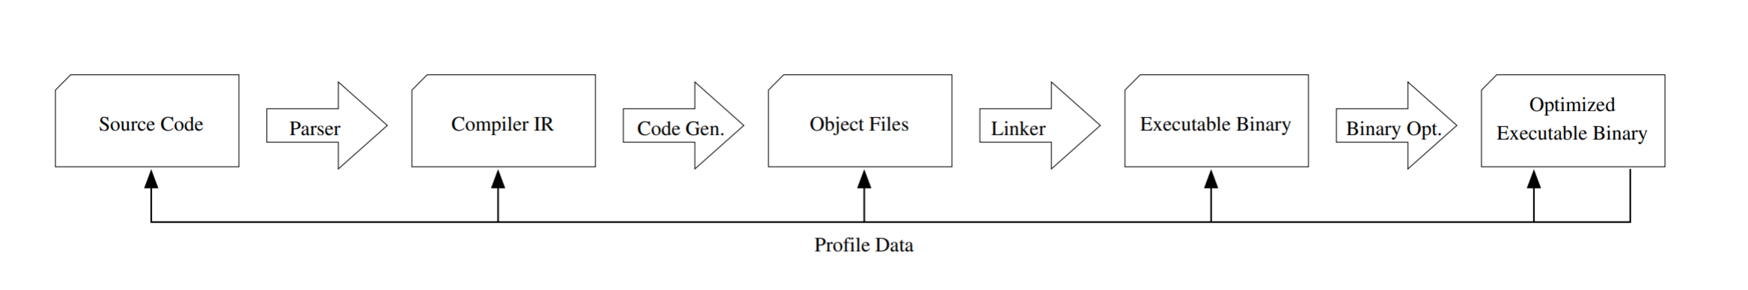
\includegraphics[width=1.0\linewidth]{translation}
    }
    \caption{Процесс трансляции исходного кода в оптимизированный бинарный файл}\label{fig:Compile}
\end{figure}

Оптимизация приложений является важнейшей частью процесса создания современного программного обеспечения, так как позволяет в разы повысить производительность и энергоэффективность вычислений. Оптимизации на основе профильной информации приложения позволяют получить большой прирост в указанных выше параметрах. Для получения профиля нужно использовать специально собранную версию приложения либо обеспечивать аппаратную поддержку сбора необходимых характеристик.

Для архитектуры x86 существует специальная аппаратная поддержка, позволяющая собирать профильную информацию во время исполнения приложения - LBR (Last Branch Record). Для ARM архитектуры аналог данной технологии существует, но не поддерживается всеми процессорами, что создаёт проблемы для оптимизаций приложений с учётом профиля исполнения. Произвести статическую инструментацию приложения не всегда является возможным, например, в случае отсутствия исходного кода или информации о символах и релокационных данных в бинарном файле. Поэтому \textbf{актуальной} задачей является разработка метода получения профильной информации для ARM архитектуры и дополнительных бинарных оптимизаций.

{\aim} данной работы является изучение и оптимизация существующих инструментов статической бинарной трансляции под RISC архитектуры. Основной целевой платформой является одна из наиболее распространенных на данный момент RISC архитектур -- ARM. Основным классом оптимизаций являются оптимизации, использующие профильную информацию исполнения приложения.

Для~достижения поставленной цели необходимо было решить следующие {\tasks}:
\begin{enumerate}[beginpenalty=10000] % https://tex.stackexchange.com/a/476052/104425
  \item Исследовать существующие статические бинарные трансляторы под RISC архитектуры.
  \item Разработать универсальный метод получения профильной информации под RISC архитектуры.
  \item Разработать ПО для получения профильной информации приложения по трассе его исполнения.
  \item Разработать методы улучшения статического бинарного транслятора.
  \item Реализовать наиболее перспективные методы улучшения бинарного оптимизатора.
  \item Разработать новые оптимизации на основе внедренных методов и улучшений.
  \item Протестировать разработанные методы на реальных приложениях под RISC архитектуру.
\end{enumerate}

Тема и содержание диссертационной работы соответствует паспорту научной специальности 05.13.11 – Математическое и программное обеспечение вычислительных машин, комплексов и компьютерных сетей, в частности, пунктам:

п. 1 – Модели, методы и алгоритмы проектирования и анализа программ и программных систем, их эквивалентных преобразований, верификации и тестирования.

п. 3 – Модели, методы, алгоритмы, языки и программные инструменты для организации взаимодействия программ и программных систем.

{\novelty}
\begin{enumerate}[beginpenalty=10000] % https://tex.stackexchange.com/a/476052/104425
  \item В диссертационной работе был реализован новый алгоритм получения профильной информации формата BOLT на основе трасс исполнения приложения. В диссертации показано, что для определенных классов устройств это единственный способ получения полноценного профиля приложения.
  \item Была реализована полноценная поддержка бинарного оптимизатора BOLT для ARM архитектуры, необходимая для проведения тестовых замеров на целевых приложениях, в то время как исходная версия BOLT не поддерживает оптимизацию нужных приложений.
  \item Был разработан специальный формат, описывающий преобразования исполняемого файла в оптимизированный.
  \item Был разработан статический анализатор, верифицирующий оптимизированный исполняемый файл на основе оригинального файла и файла преобразования.
  \item Был создан алгоритм мультипрофильного анализа, выделяющий профили приложения на основе трасс исполнения. На его основе реализована оптимизация копирования кода.

\end{enumerate}

{\influence} данной работы заключается в использовании разработанных методов и алгоритмов в бинарном оптимизаторе BOLT и его инфраструктуре и успешном \textbf{внедрении} компанией ООО <<Техкомпания Хуавэй>> для оптимизации приложений. Реализованные оптимизации, верификации и методы получения профильной информации позволили получить прирост производительности на целевых приложениях компании.

Результаты данной работы также \textbf{внедрены} в кафедральный курс «Современные методы разработки компиляторов» кафедры микропроцессорных технологий в интеллектуальных системах управления МФТИ.

Теоретическая значимость диссертационной работы заключается в разработке новых методов использования трасс исполнения приложения, как для получения профильной информации, так и для использования в анализе и оптимизациях.

{\defpositions}
\begin{enumerate}[beginpenalty=10000] % https://tex.stackexchange.com/a/476052/104425
  \item Метод получения профильной информации для бинарного оптимизатора BOLT из трасс исполнения приложений.
  \item Алгоритм оптимизации длинных переходов при работе бинарного оптимизатора BOLT.
  \item Алгоритм верификации оптимизированных бинарным оптимизатором BOLT файлов.
  \item Алгоритм мультипрофильного анализа трасс исполнения приложений.
  \item Алгоритм дублирования кода на основе мультипрофильного анализа трасс исполнения приложений.
\end{enumerate}

{\reliability}
Обоснованность и достоверность результатов и выводов диссертации подтверждается подробным описанием проведенных экспериментов и полученных данных.

{\probation}
Результаты диссертационной работы докладывались на следующих научно-технических конференциях:
\begin{enumerate}[beginpenalty=10000] % https://tex.stackexchange.com/a/476052/104425
  \item 63-й всероссийской научной конференции московского физико–технического института (государственного университета, Москва, ноябрь 2020 г.
  \item Международном конгрессе <<Современные проблемы компьютерных и информационных наук>>, Москва, ноябрь 2021 г.
  \item 64-й всероссийской научной конференции московского физико–технического института (государственного университета, Москва, ноябрь 2021 г.
\end{enumerate}

{\contribution} Основные результаты диссертационного исследования получены лично автором. Постановка задач и анализ полученных результатов осуществлялся непосредственно автором. В совместных работах вклад автора в результаты исследования являлся определяющим. Автор лично реализовывал и интегрировал разработанные решения в бинарный оптимизатор BOLT.

\ifnumequal{\value{bibliosel}}{0}
{%%% Встроенная реализация с загрузкой файла через движок bibtex8. (При желании, внутри можно использовать обычные ссылки, наподобие `\cite{vakbib1,vakbib2}`).
    {\publications} Основные результаты по теме диссертации изложены
    в~XX~печатных изданиях,
    X из которых изданы в журналах, рекомендованных ВАК,
    X "--- в тезисах докладов.
}%
{%%% Реализация пакетом biblatex через движок biber
    \begin{refsection}[bl-author, bl-registered]
        % Это refsection=1.
        % Процитированные здесь работы:
        %  * подсчитываются, для автоматического составления фразы "Основные результаты ..."
        %  * попадают в авторскую библиографию, при usefootcite==0 и стиле `\insertbiblioauthor` или `\insertbiblioauthorgrouped`
        %  * нумеруются там в зависимости от порядка команд `\printbibliography` в этом разделе.
        %  * при использовании `\insertbiblioauthorgrouped`, порядок команд `\printbibliography` в нём должен быть тем же (см. biblio/biblatex.tex)
        %
        % Невидимый библиографический список для подсчёта количества публикаций:
        \printbibliography[heading=nobibheading, section=1, env=countauthorvak,          keyword=biblioauthorvak]%
        \printbibliography[heading=nobibheading, section=1, env=countauthorwos,          keyword=biblioauthorwos]%
        \printbibliography[heading=nobibheading, section=1, env=countauthorscopus,       keyword=biblioauthorscopus]%
        \printbibliography[heading=nobibheading, section=1, env=countauthorconf,         keyword=biblioauthorconf]%
        \printbibliography[heading=nobibheading, section=1, env=countauthorother,        keyword=biblioauthorother]%
        \printbibliography[heading=nobibheading, section=1, env=countregistered,         keyword=biblioregistered]%
        \printbibliography[heading=nobibheading, section=1, env=countauthorpatent,       keyword=biblioauthorpatent]%
        \printbibliography[heading=nobibheading, section=1, env=countauthorprogram,      keyword=biblioauthorprogram]%
        \printbibliography[heading=nobibheading, section=1, env=countauthor,             keyword=biblioauthor]%
        \printbibliography[heading=nobibheading, section=1, env=countauthorvakscopuswos, filter=vakscopuswos]%
        \printbibliography[heading=nobibheading, section=1, env=countauthorscopuswos,    filter=scopuswos]%
        %
        \nocite{*}%
        %
        {\publications} Основные результаты по теме диссертации изложены в~\arabic{citeauthor}~печатных изданиях,
        \arabic{citeauthorvak} из которых изданы в журналах, рекомендованных ВАК\sloppy%
        \ifnum \value{citeauthorscopuswos}>0%
            , \arabic{citeauthorscopuswos} "--- в~периодических научных журналах, индексируемых Web of~Science и Scopus\sloppy%
        \fi%
        \ifnum \value{citeauthorconf}>0%
            , \arabic{citeauthorconf} "--- в~тезисах докладов.
        \else%
            .
        \fi%
        \ifnum \value{citeregistered}=1%
            \ifnum \value{citeauthorpatent}=1%
                Зарегистрирован \arabic{citeauthorpatent} патент.
            \fi%
            \ifnum \value{citeauthorprogram}=1%
                Зарегистрирована \arabic{citeauthorprogram} программа для ЭВМ.
            \fi%
        \fi%
        \ifnum \value{citeregistered}>1%
            Зарегистрированы\ %
            \ifnum \value{citeauthorpatent}>0%
            \formbytotal{citeauthorpatent}{патент}{}{а}{}\sloppy%
            \ifnum \value{citeauthorprogram}=0 . \else \ и~\fi%
            \fi%
            \ifnum \value{citeauthorprogram}>0%
            \formbytotal{citeauthorprogram}{программ}{а}{ы}{} для ЭВМ.
            \fi%
        \fi%
        % К публикациям, в которых излагаются основные научные результаты диссертации на соискание учёной
        % степени, в рецензируемых изданиях приравниваются патенты на изобретения, патенты (свидетельства) на
        % полезную модель, патенты на промышленный образец, патенты на селекционные достижения, свидетельства
        % на программу для электронных вычислительных машин, базу данных, топологию интегральных микросхем,
        % зарегистрированные в установленном порядке.(в ред. Постановления Правительства РФ от 21.04.2016 N 335)
    \end{refsection}%
    \begin{refsection}[bl-author, bl-registered]
        % Это refsection=2.
        % Процитированные здесь работы:
        %  * попадают в авторскую библиографию, при usefootcite==0 и стиле `\insertbiblioauthorimportant`.
        %  * ни на что не влияют в противном случае
        \nocite{vakbib1}%vak
        \nocite{vakbib2}%vak
        \nocite{confbib1}%conf
        \nocite{confbib2}%conf
        \nocite{confbib3}%conf
    \end{refsection}%
        %
        % Всё, что вне этих двух refsection, это refsection=0,
        %  * для диссертации - это нормальные ссылки, попадающие в обычную библиографию
        %  * для автореферата:
        %     * при usefootcite==0, ссылка корректно сработает только для источника из `external.bib`. Для своих работ --- напечатает "[0]" (и даже Warning не вылезет).
        %     * при usefootcite==1, ссылка сработает нормально. В авторской библиографии будут только процитированные в refsection=0 работы.
} % Характеристика работы по структуре во введении и в автореферате не отличается (ГОСТ Р 7.0.11, пункты 5.3.1 и 9.2.1), потому её загружаем из одного и того же внешнего файла, предварительно задав форму выделения некоторым параметрам

%Диссертационная работа была выполнена при поддержке грантов \dots

%\underline{\textbf{Объем и структура работы.}} Диссертация состоит из~введения,
%четырех глав, заключения и~приложения. Полный объем диссертации
%\textbf{ХХХ}~страниц текста с~\textbf{ХХ}~рисунками и~5~таблицами. Список
%литературы содержит \textbf{ХХX}~наименование.

\pdfbookmark{Содержание работы}{description}                          % Закладка pdf
\section*{Содержание работы}
\underline{\textbf{Введение}} содержит обоснование актуальности
исследований, проводимых в~рамках данной диссертационной работы,
обзор научной литературы по~изучаемой проблеме, а также формулируется цель, ставятся задачи, излагается научная новизна
и практическая значимость представляемой работы. 

\begin{figure}[!h]
    \centerfloat{
        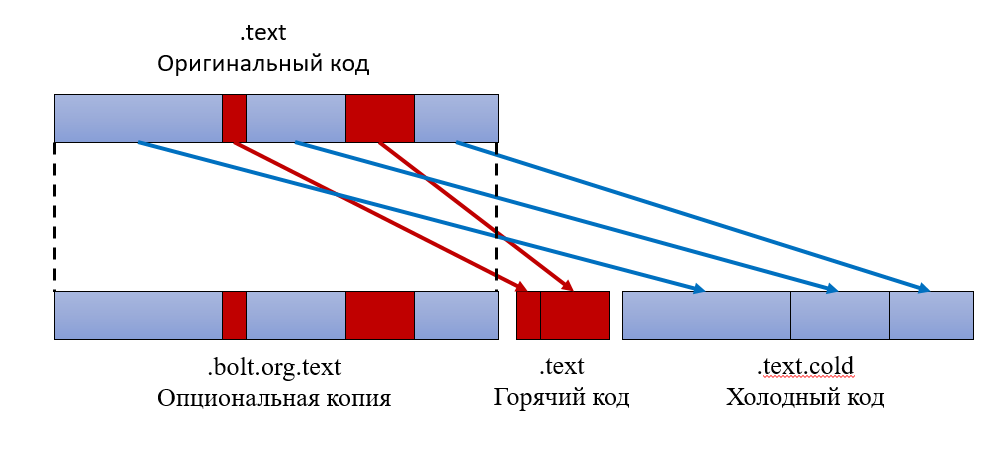
\includegraphics[width=1.0\linewidth]{1}
    }
    \caption{Алгоритм работы бинарного оптимизатора BOLT}\label{fig:BOLT}
\end{figure}

\underline{\textbf{Первая глава}} посвящена обзору существующих технологий бинарных трансляторов, используемых для генерации оптимизированных исполняемых файлов приложений. В начале главы приводится принятая классификация современных бинарных трансляторов. Затем рассматриваются общие принципы работы существующих технологий бинарной оптимизации. Далее описывается схема работы бинарных оптимизаторов, использующих  профильную информацию исполнения приложения.

Приводится описание работы бинарного оптимизатора BOLT (Binary Optmization and Layout Tool) (рисунки \cref{fig:BOLT} и \cref{fig:BinOpt}). Обсуждаются вопросы получения профильной информации для его работы на x86 архитектуре с использованием аппаратной поддержки профилирования -- LBR (Last Branch Record)  (рисунок \cref{fig:BinOptX86}). Также рассматривается альтернативный вариант сбора профильной информации без аппаратной поддержки сбора статистики  переходов -- режим работы no\_LBR\_mode. В нём собирается только статистика исполняемых адресов в бинарном файле.

\begin{figure}[!h]
    \centerfloat{
        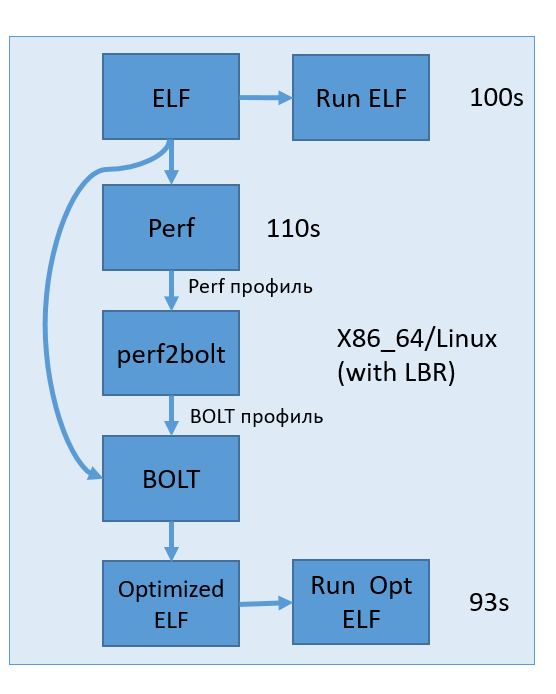
\includegraphics[width=0.5\linewidth]{2}
    }
    \caption{Схема оптимизации бинарного файла на x86 архитектуре}\label{fig:BinOptX86}
\end{figure}

Кроме того, подробно рассматриваются вопросы формата профилей с информацией о взятых переходах и без неё. Разбирается пример оптимизации простого приложения с условным переходом в цикле. Приводится его граф потока управления и варианты раскладки  его бинарного кода в памяти.

\begin{figure}[!h]
    \centerfloat{
        
\includegraphics[width=1.0\linewidth]{3}
    }
    \caption{Последовательность работы бинарного оптимизатора BOLT}\label{fig:BinOpt}
\end{figure}

В конце первой главы рассматривается вопрос поддержки архитектуры ARM в бинарном оптимизаторе BOLT, варианты получения профильной информации на ней и возможности оптимизаций, приведены примеры профилей в формате BOLT.

\underline{\textbf{Вторая глава}} посвящена разработанному универсальному методу получения профильной информации приложения из трасс исполнения.

В \underline{\textbf{разделе 2.1}} описывается метод получения трасс исполнения приложений на основе динамической бинарной инструментации (DBI, Dynamic Binary Instrumentation) и предлагается схема оптимизации бинарного файла на ARM архитектуре (рисунок \cref{fig:SugOpt}).

\begin{figure}[!h]
    \centerfloat{
        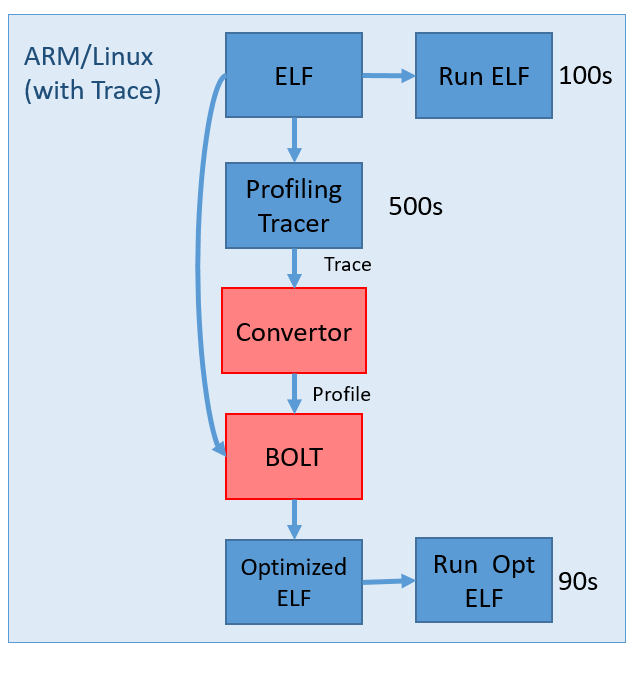
\includegraphics[width=0.6\linewidth]{9}
    }
    \caption{Предлагаемая схема оптимизации бинарного файла на ARM архитектуре}\label{fig:SugOpt}
\end{figure}

С помощью DBI фреймворка производится запись трассы исполнения приложения. Записывается последовательность инструкций, поступающих на процессор. После исполнения последовательность анализируется конвертером для генерации профиля исполнения, который записывается в формате BOLT. Такое решение приводит к замедлению работы оптимизируемого приложения в несколько раз, но создаёт трассу, которую можно анализировать без привязки к конкретной микроархитектуре.

В \underline{\textbf{разделе 2.2}} изложен алгоритм работы модели предсказателя переходов по трассе исполнения приложения, необходимый для получения информации о промахах предсказателя для профиля (рисунок \cref{fig:ProfTrace}).

\begin{figure}[!h]
    \centerfloat{
        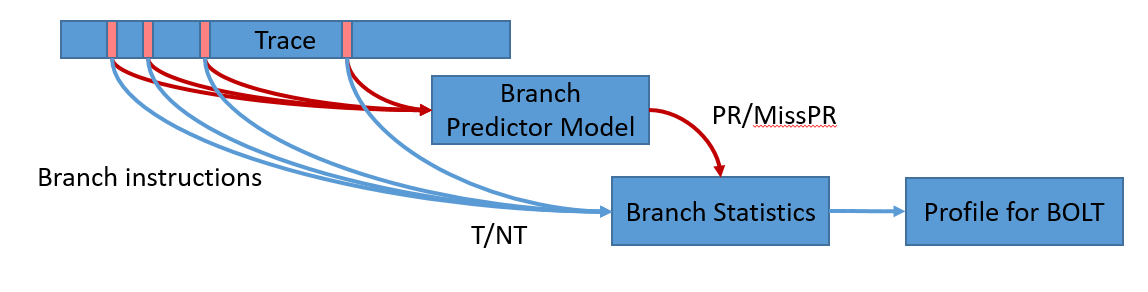
\includegraphics[width=1.0\linewidth]{10}
    }
    \caption{Схема генерации профиля из трассы исполнения}\label{fig:ProfTrace}
\end{figure}

Для получения информации о переходах для профиля конвертер проходит по всей трассе и находит инструкции, меняющие поток управления: B, BR, BL, BLR, B.cond, TBZ, TBNZ, CBZ, CBNZ, RET. После этого информация поступает в модель предсказателя переходов (Branch Predictor Model). Данная модель выбирается в зависимости от конкретной микроархитектуры процессора, для которого оптимизируется приложение. В итоге собирается информация для получения количества не предсказанных и количества взятых переходов.

В \underline{\textbf{разделе 2.3}} приводится сравнение предлагаемого решения с уже существующим подходом работы бинарного оптимизатора BOLT. Сопоставляются профили, полученные на ARM и x86 архитектурах. Метод сбора профильной информации с использованием трассы исполнения был проверен на приложениях, собранных под архитектуру ARM. Для аналогичных программ под x86 собранные с помощью LBR профили коррелируют с полученными, что позволяет использовать динамическую бинарную инструментацию с последующим анализом переходов для использования с оптимизатором BOLT.

Помимо этого, сравниваются подходы получения профильной информации с помощью аппаратной поддержки LBR и получение из трасс исполнения приложения. Во-первых, трасса исполнения зависит только от архитектуры, но не микроахитетктуры устройства, на котором происходит динамическая бинарная инструментация, что означает возможность повторной оптимизации приложения под другую микроахитектуру с другой моделью предсказателя переходов. Во-вторых, собранный профиль покрывает всё исполнение оптимизируемого приложения, а не часть исполнения как в случае с LBR. Таким образом, полученная информация более корректна, так как избавляет профиль от искажений, связанных с ожиданием готовности периферии процессора, например, обращение в память.

В \underline{\textbf{разделе 2.4}} описываются используемые синтетические тесты для проверки корректности работы предлагаемого метода получения профильной информации.

Искусственно были созданы примеры, когда исполняемый код перемешан с не исполняемым холодным кодом, что приводит к неэффективному использованию инструкционного кэша. Для генерации бинарного файла большого размера (> 10 МБ) применялись рекурсивный вызов шаблонных функций в языке программирования C++. С их помощью компилятор создавал множественные копии функций с разными шаблонными константами, тем самым увеличивая размер кода до нужного значения. Исполняемый код равномерно распределяется по секции, чередуясь с холодными функциями. 

В \underline{\textbf{разделе 2.5}} приводятся результаты запусков, оптимизированных на основе профильной информации, которая была собрана из трасс исполнения синтетических тестов.

\begin{figure}[H]
    \centerfloat{
        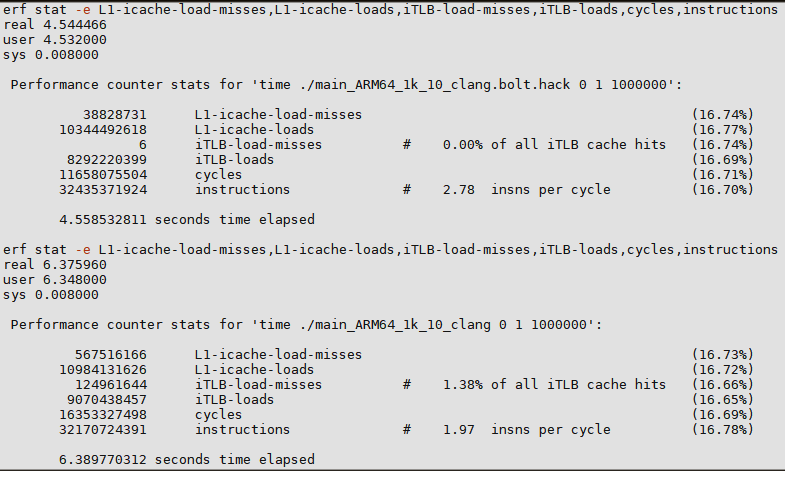
\includegraphics[width=1.0\linewidth]{13}
    }
    \caption{Сравнение результатов запусков оригинального (снизу) и оптимизированного (сверху) бинарных файлов синтетического теста}\label{fig:SynthRes}
\end{figure}

Полученные статистические данные  (рисунок \cref{fig:SynthRes}) показывают понижение практически до нуля количество промахов по iTLB, увеличение IPC (instruction per clock) на 41\% и уменьшение времени работы на 29\%. Для тестирования была выбрана микроархитектура ARM Cortex A76.

\underline{\textbf{Третья глава}} посвящена описанию улучшений в бинарном оптимизаторе BOLT под ARM архитектуру, их верификации и тестированию.

В \underline{\textbf{разделе 3.1}} рассматривается проблема длинных переходов в бинарной оптимизации. Описывается метод оптимизации трамплинов, позволяющий уменьшить количество добавляемых для трамплина инструкций и не использовать дополнительный регистр.

Перекомпоновка кода проще реализуется на CISC архитектуре за счёт возможности добавления длинных прыжков одной инструкцией. На RISC архитектурах количество битов смещения в инструкциях переходов меньше, что приводит к ограничению диапазона возможного перемещения. Также инструкция загрузки в регистр адреса, зависящего от счетчика инструкций, на ARM архитектуре ограничена 20 битами, выделенными на смещение, и накладывает возможный диапазон перемещения ± 1 мегабайт. Все инструкции, которые зависят от своего адреса (переходы, загрузка адреса, загрузка по регистру/смещению), после оптимизации необходимо проверить на возможность записи нового смещения в отведенные для этого биты.

\begin{figure}[H]
    \centerfloat{
        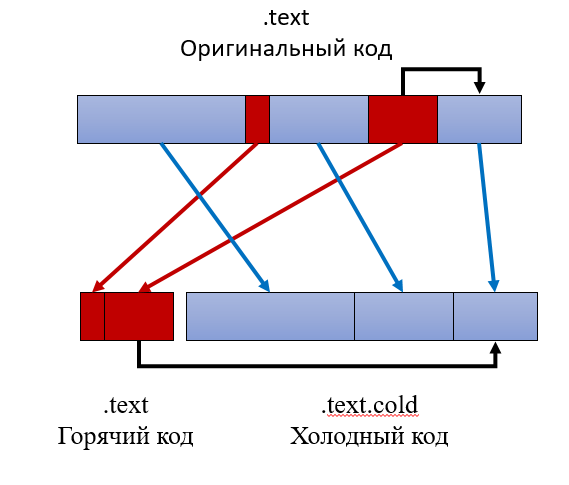
\includegraphics[width=0.8\linewidth]{11}
    }
    \caption{Пример перекомпоновки кода}\label{fig:HotMove}
\end{figure}

Таким образом, при перемещении горячего кода, ссылающегося на холодный участок (черная стрелка на рисунке \cref{fig:HotMove}), происходит переполнение значения смещения, и оптимизация становится некорректной.

Для решения данной проблемы необходимо добавить трамплин – дополнительный код, позволяющий генерировать произвольный адрес и произвести переход либо загрузку по данному значению. Подобное решение будет увеличивать размер кода, что приведёт к понижению производительности, но диапазон перемещаемого кода будет увеличен.

\begin{figure}[!h]
    \centerfloat{
        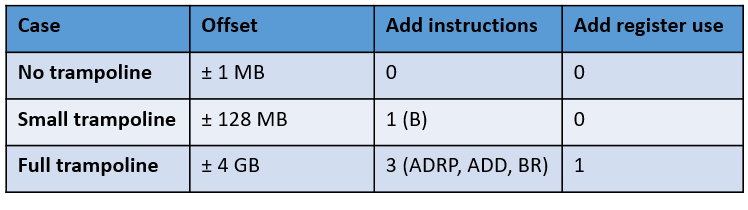
\includegraphics[width=1.0\linewidth]{opt4}
    }
    \caption{Сравнение трамплинов}\label{fig:CompTramp}
\end{figure}

Для условных переходов можно написать маленькие трамплины размером в одну инструкцию с помощью добавления одного безусловного перехода в случае, если смещение занимает больше 19, но меньше 26 бит (рисунок \cref{fig:CompTramp}).
 
\begin{figure}[H]
    \centerfloat{
        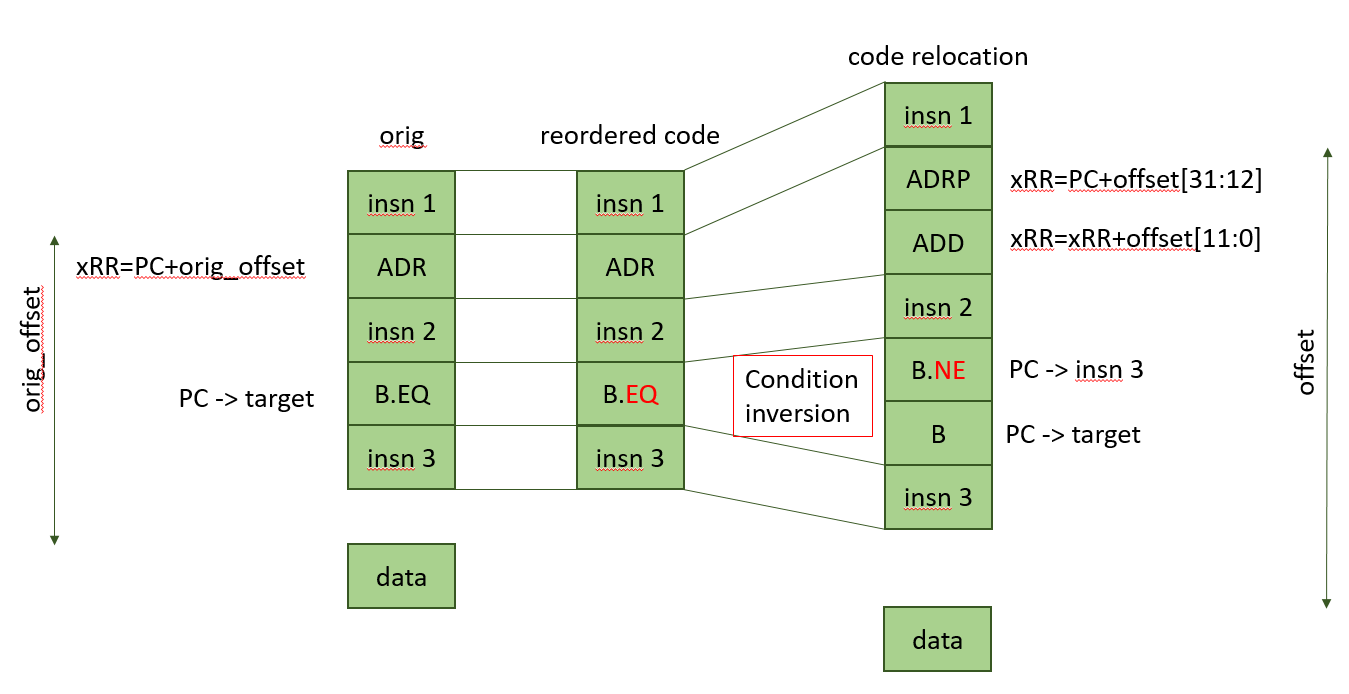
\includegraphics[width=1.0\linewidth]{opt2}
    }
    \caption{Схема добавления трамплинов для ADR (сверху) и Bcc (снизу) инструкций}\label{fig:Tramp}
\end{figure}

В данном варианте необходимо инвертировать условие инструкции и метку для прыжка поставить через одну инструкцию прямого перехода, вставленную оптимизатором непосредственно после условного перехода. Получаем увеличение возможного региона перемещения в 128 раз за счёт отличий в кодировках Bcc и B, а увеличение кода произошло всего на 1 инструкцию (рисунок \cref{fig:Tramp}).

В \underline{\textbf{разделе 3.2}} описывается проблема бинарной оптимизации исполняемых файлов под ARM архитектуру, в которых используются таблицы переходов.

\begin{figure}[!h]
    \centerfloat{
        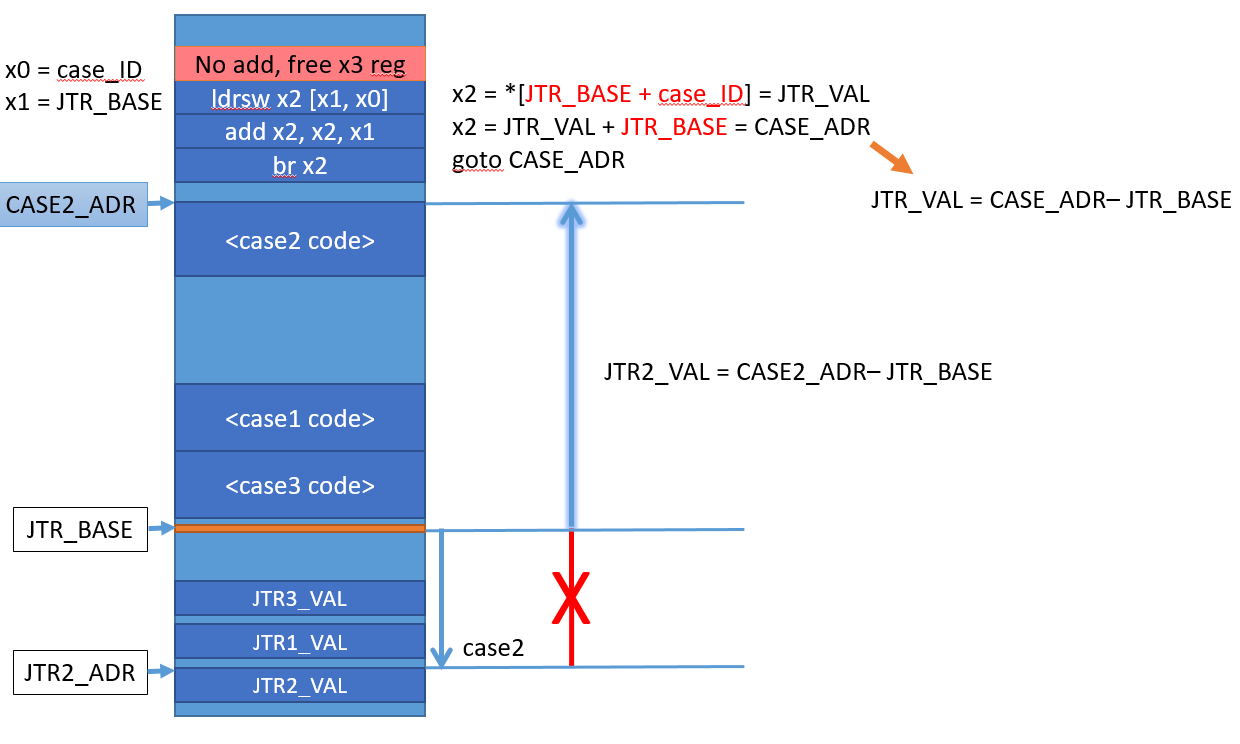
\includegraphics[width=1.0\linewidth]{jt4}
    }
    \caption{Оптимизированный вариант ассемблерного кода для switch-case случая}\label{fig:Switch}
\end{figure}

При перемещении кода конкретного варианта конструкции switch-case, необходимо модифицировать запись в таблице, используемую в косвенном переходе. Оптимизатор узнает адрес записи из релокационной информации, которая для некоторых случаев кода ARM архитектуры не будет корректной (рисунок \cref{fig:Switch}). Это происходит по причине несоответствия адреса, от которого вычисляется целевой адрес для прыжка при исполнении и генерации релокационной информации.

Данная проблема решается переиспользованием оригинального участка кода с данным косвенным переходом. В этом случае необходимо сохранить копию оригинальной секции .bolt.org.text.

В \underline{\textbf{разделе 3.3}} предлагается метод верификации оптимизированного бинарного файла.

Для решения данной задачи был разработан специальный формат, описывающий преобразования исполняемого файла в оптимизированный, так называемый remap-файл. В нём записывается информация о всех совершенных перестановках кода и дополнительная информация, обозначающая инструкции, подвергнутые преобразованиям в процессе перекомпоновки (PC-relative инструкции).

\begin{figure}[!h]
    \centerfloat{
        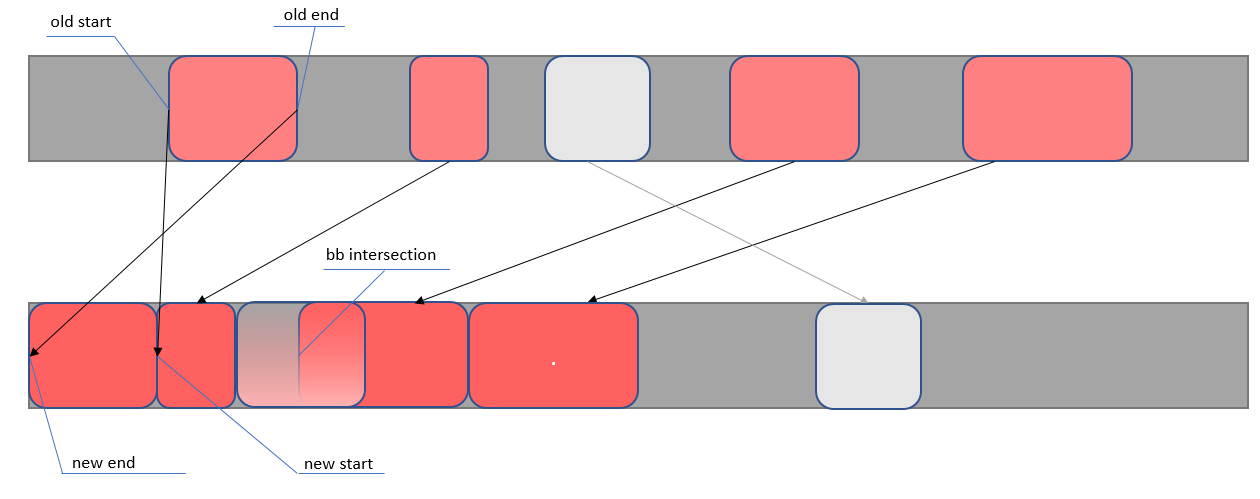
\includegraphics[width=1.0\linewidth]{v2}
    }
    \caption{Схема верификации бинарного файла}\label{fig:Verif}
\end{figure}

В рамках данной работы в оптимизатор BOLT был добавлен проход, генерирующий remap-файл, а также написан статический анализатор, сравнивающий оригинальный и оптимизированный исполняемые файлы по данному remap-файлу (рисунок \cref{fig:Verif}). Реализованы следующие проверки:

\begin{enumerate}[beginpenalty=10000]
  \item Проверка корректности оптимизированных линейных участков кода.
  \item Проверка корректности создания теневых точек.
  \item Сравнение инструкций оптимизированных и исходный линейных участков.
\end{enumerate}	

В \underline{\textbf{разделе 3.4}} описываются результаты тестирования синтетических тестов и общих наборов тестов после оптимизации модифицированным бинарным транслятором BOLT (рисунки \cref{fig:OrigClang} и \cref{fig:OptClang}).

Для проверки оптимизации на реальном приложении был выбран набор тестов производительности GeekBench. Среди всего набора был выбран тест с наибольшим числом iTLB и L1I промахов – Clang. При компиляции набора тестов были использован флаг <<-O2>>, который соответствует оптимизациям при стандартной сборке приложений.

По результатам тестов был получен прирост в показателях теста на 10\%, уменьшение iTLB и L1I промахов на 32\% и 38\% соответственно, что является показателем увеличения средней температуры кода. При этом остальные тесты из набора GeekBench либо не улучшили производительность, либо ухудшили её.

\begin{figure}[H]
    \centerfloat{
        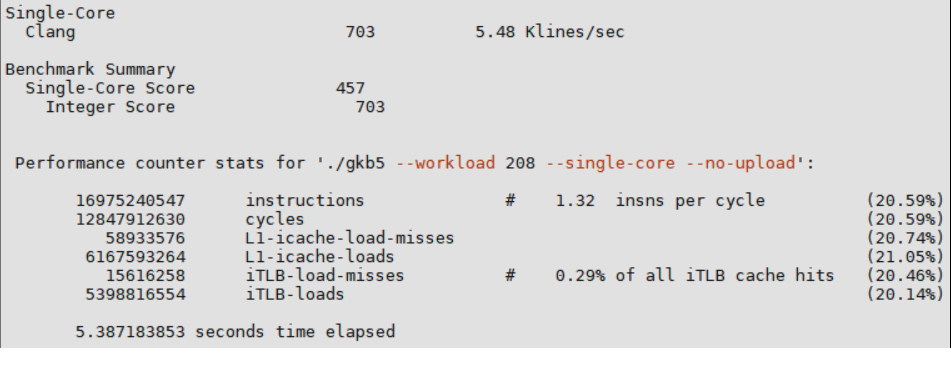
\includegraphics[width=1.0\linewidth]{14}
    }
    \caption{Результаты исполнения оригинального Clang теста}\label{fig:OrigClang}
\end{figure}

\begin{figure}[H]
    \centerfloat{
        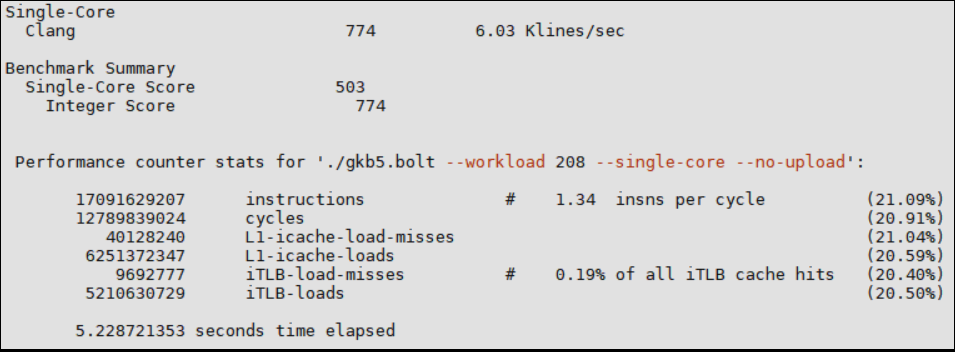
\includegraphics[width=1.0\linewidth]{15}
    }
    \caption{Результаты исполнения оптимизированного Clang теста}\label{fig:OptClang}
\end{figure}

В \underline{\textbf{четвертой главе}} приведено описание бинарных оптимизаций на основе трасс исполнения приложения.

В \underline{\textbf{разделе 4.1}} описываются проблемы оптимизаций с профильной информацией.

Для работы оптимизатора BOLT необходимы значения счетчика команд и последние взятые переходы с информацией от предсказателя переходов. Во время сбора характеристик программа исполняется по определенному сценарию: определенные входные данные, параметры окружения, контекст и т.д. Полученная профильная информация будет показывать характеристики этого выбранного сценария.

После оптимизации приложения с данным профилем запуск по данному сценарию будет показывать прирост производительности, но при проверке производительности с другими входными параметрами на данном приложении такого же прироста производительности получить не удастся (вероятно будет происходить регрессия).

Кроме того, приводится пример приложения, при оптимизации которого будет получен либо прирост, либо регрессия производительности в зависимости от выбранного сценария.

В \underline{\textbf{разделе 4.2}} рассматривается дополнительная информация, которую можно извлечь из трассы исполнения и применить для последующей бинарной оптимизации приложения.

Трасса исполнения содержит в себе гораздо больше информации, чем профиль, который в конечном итоге используется для оптимизации приложения. Помимо количества сделанных переходов на каждой инструкции и изменения программного счетчика, есть информация о последовательности сделанных переходов, которую можно учитывать во время оптимизации.

Также для оптимизации можно добавить в трассу информацию про использованные адреса в инструкциях загрузки и выгрузки. Таким образом, можно достать подробную информацию для оптимизации данных в бинарном файле.

В \underline{\textbf{разделе 4.3}} приводится описание мультипрофильного анализа трасс исполнения приложения. Вводятся основные необходимые термины для данного анализа: интервалы инструкций, фазы исполнения и мультипрофиль.

Трасса разбивается на одинаковые интервалы по количеству инструкций. Это необходимо для анализа исполнения в рамках одного отрезка времени – интервала инструкций, так как требуется найти похожие интервалы и объединить их в фазы.

Для большей наглядности граф исполнения отображается в виде тепловой карты (рисунок \cref{fig:HeatMap}). По оси X – интервалы инструкций согласно времени исполнения, по оси Y – номер линейного участка кода.

\begin{figure}[!h]
    \centerfloat{
        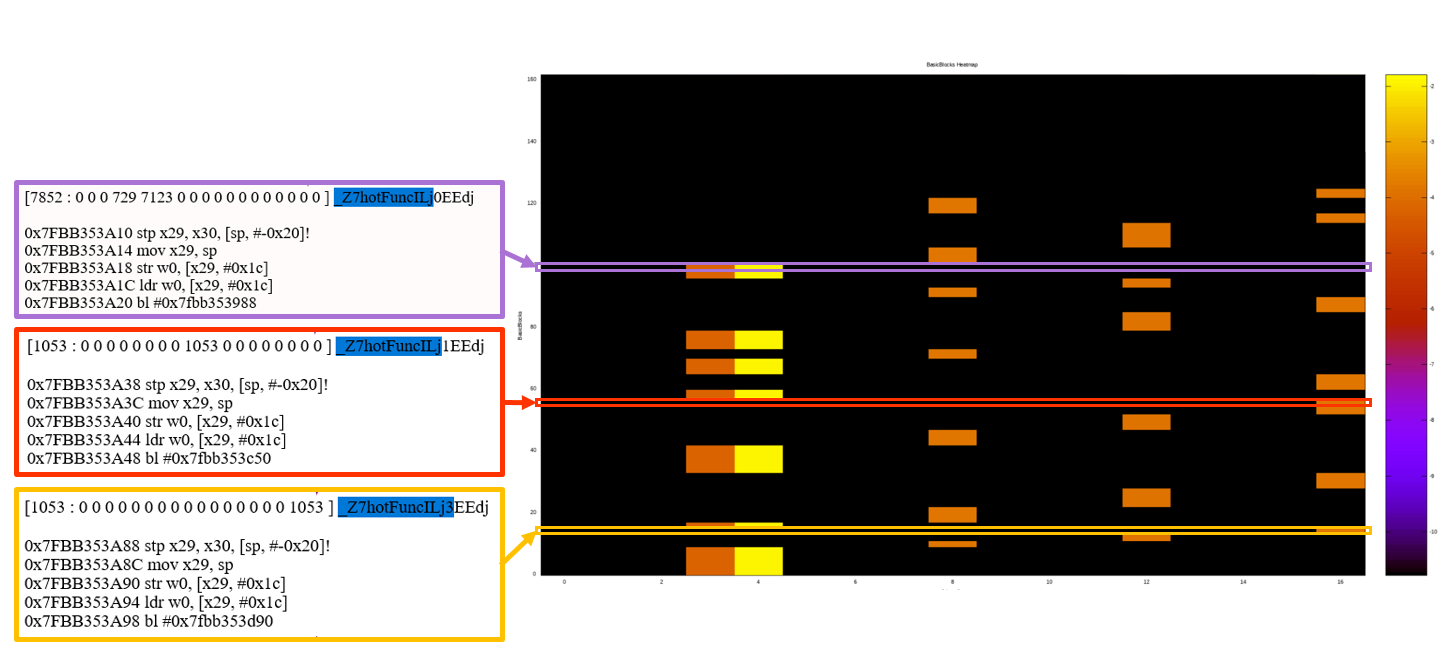
\includegraphics[width=1.0\linewidth]{_9}
    }
    \caption{Построение тепловой карты линейных участков}\label{fig:HeatMap}
\end{figure}

На каждом интервале исполнялся определенный набор линейных участков кода, который будет характеризовать интервал инструкций. Если составить n-мерное пространство, где n – количество линейных участков кода, а координаты – количество исполненных соответствующих линейных участков на выбранном интервале, то каждому интервалу в данном пространстве будет соответствовать точка.

Также в разделе приводится алгоритм кластеризации интервалов. Каждый полученный кластер интервалов инструкций означает определенную фазу. Кластеризация проводится с помощью итеративного алгоритма объединения фаз. По переключениям между фазами строится граф исполнения. Он является аналогом графа потока управления, но на более высоком уровне, показывая переключения не между линейными участками, а между макросостояниями исполнения программы.

\begin{figure}[H]
    \begin{minipage}[b][][b]{1.0\linewidth}\centering
        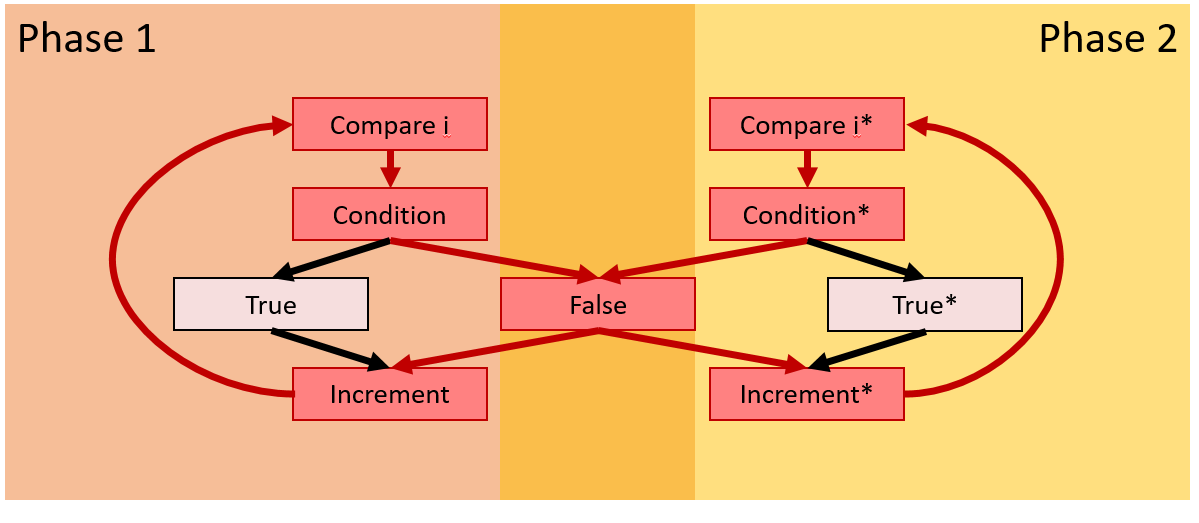
\includegraphics[width=0.8\linewidth]{mi1} \\ а)до оптимизации
    \end{minipage}
    \vfill
    \begin{minipage}[b][][b]{1.0\linewidth}\centering
        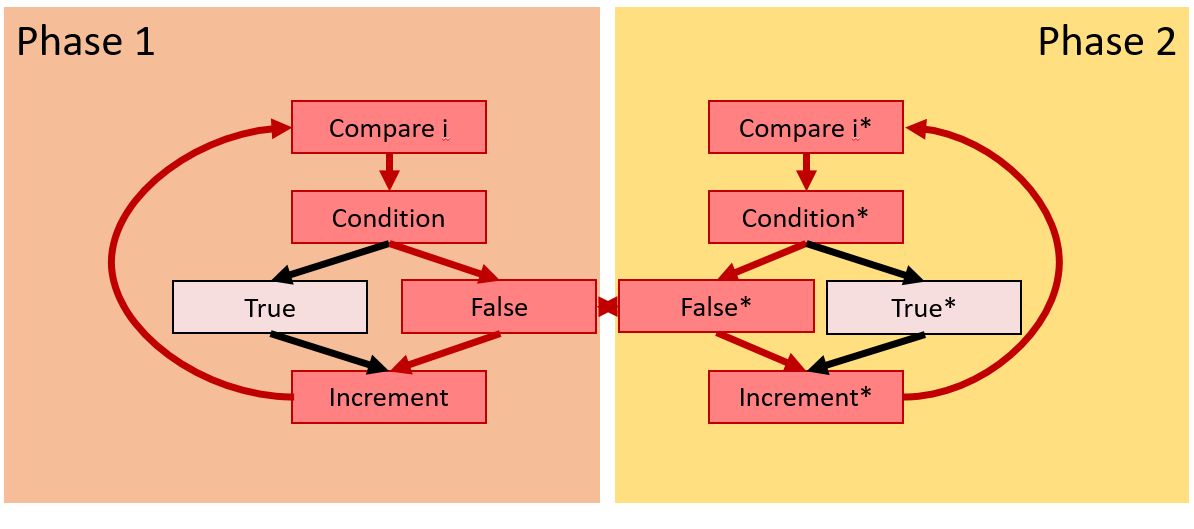
\includegraphics[width=0.8\linewidth]{mi2} \\ б)после оптимизации
    \end{minipage}
    \caption{Дублирование кода на основе мультипрофиля}
    \label{fig:MultiProfileOpt}
\end{figure}

Для завершения анализа приложения необходимо построить соответствие между фазами и линейными участками приложения. Для этого каждый линейный участок анализируется отдельно, выбирая интервал с его наибольшим количеством исполнений. Линейному участку кода будет соответствовать фаза, которая включает в себя этот интервал.

В \underline{\textbf{разделе 4.4}} описывается бинарная оптимизация - дублирование кода на основе мультипрофиля.

Выстраивая соответствие между линейными участками кода и фазами, выбиралась фаза, к которой принадлежит интервал инструкций с наибольшим количеством исполнений данного линейного участка. Однако, может произойти ситуация, когда линейный участок исполнялся на интервалах инструкций, относящихся к разным фазам. В этом случае необходимо запоминать такие линейные участки для последующего анализа необходимости дублирования данного кода.

Используя эвристически подобранные соотношения, выбираются те линейные участки, которые относятся одновременно к нескольким фазам. После этого данные участки помечаются для дублирования бинарным оптимизатором BOLT (рисунок \cref{fig:MultiProfileOpt}).

В \underline{\textbf{разделе 4.5}} приводятся результаты запусков тестов, оптимизированных с помощью дублирования кода на основе мультипрофиля.

Для проверки анализа был использован набор тестов GeekBench. Были записаны трассы его исполнения на различных задачах. На тепловой карте (рисунок \cref{fig:HeatmapGKB}) выделены запуски различных задач, представляющие в данном случае сценарии запуска приложения. По верхней строке тепловой карты видно корректное выделение фаз на каждую отдельный тест из набора.

\begin{figure}[!h]
    \centerfloat{
        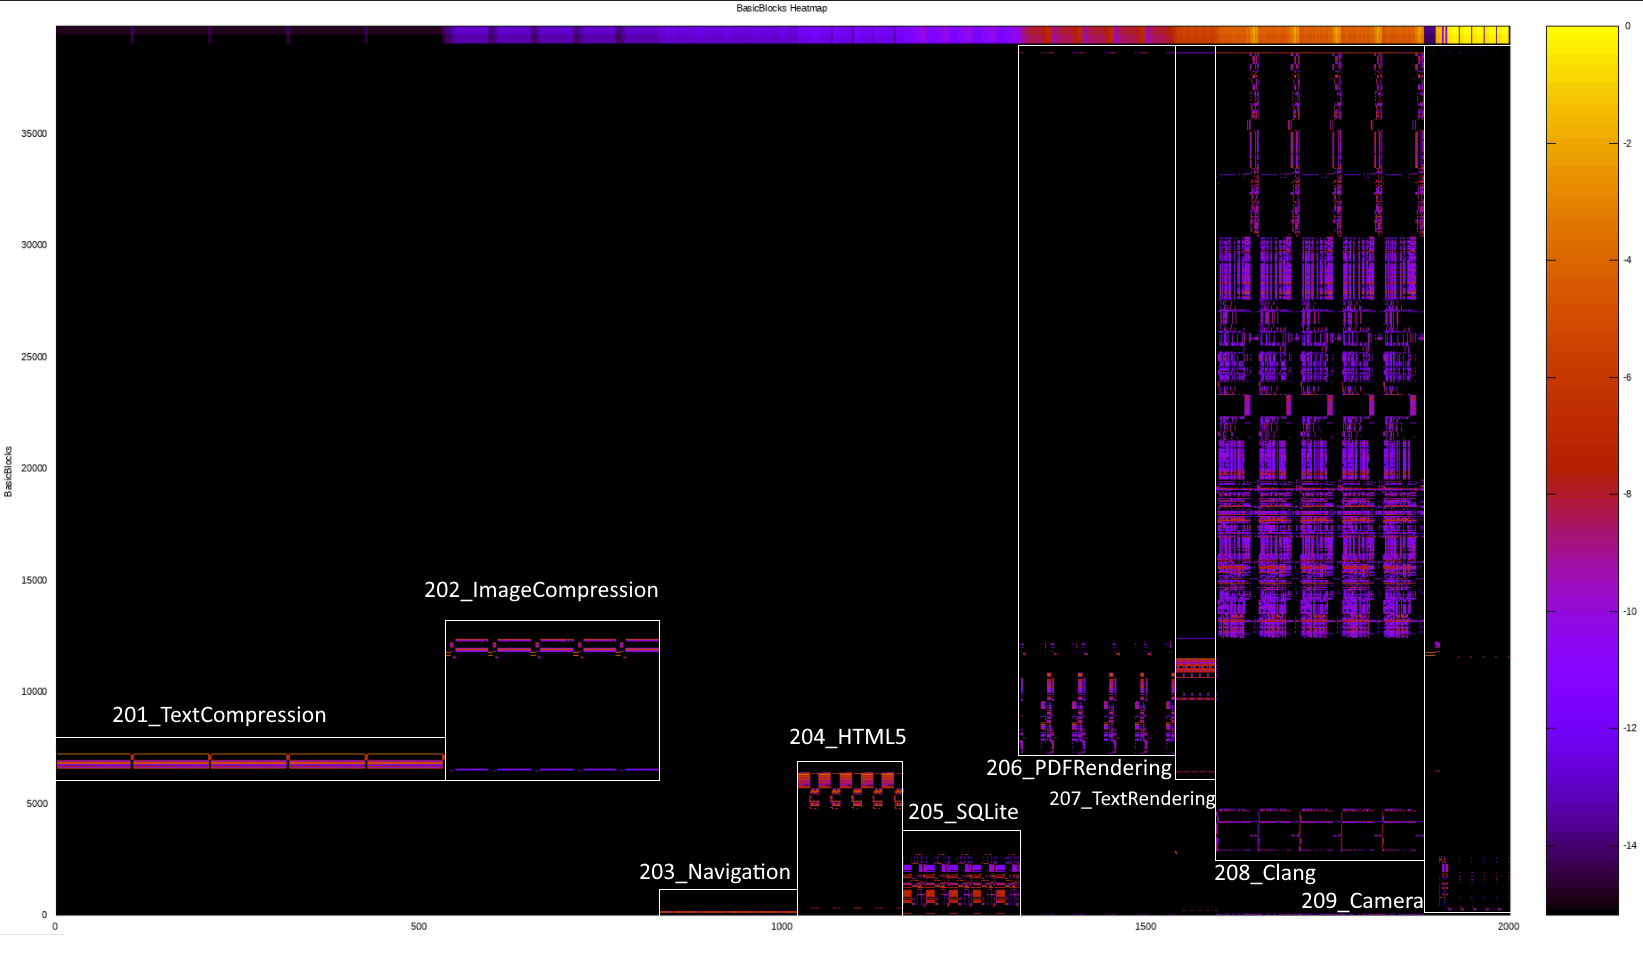
\includegraphics[width=1.0\linewidth]{_16}
    }
    \caption{Тепловая карта набора тестов Geekbench с выделенными тестами}\label{fig:HeatmapGKB}
\end{figure}

При использовании оптимизации дублирования кода на основе мультипрофильной информации удалось получить прирост производительности до 4\% на отдельных тестах из набора, но средний прирост на всех тестах не превышает 1\% (рисунок \cref{fig:ResGKB}). Это связано с отсутствием больших пересечений в коде набора тестов. Максимальный прирост был получен на мультипрофиле с 12 фазами, что коррелирует с порядком количества тестов в наборе.

\begin{figure}[!h]
    \centerfloat{
        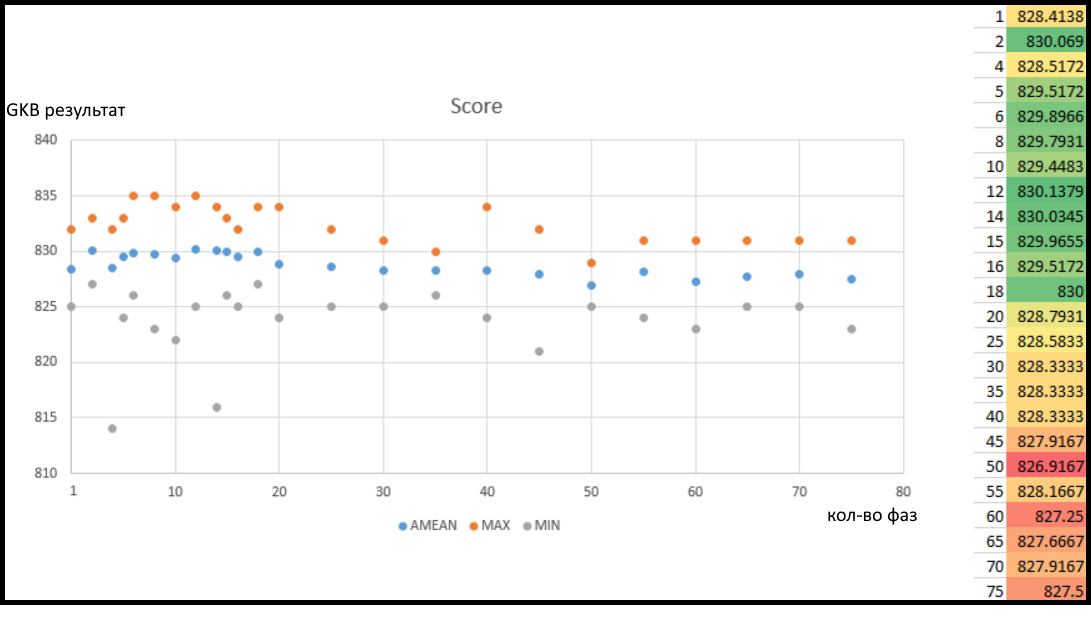
\includegraphics[width=1.0\linewidth]{scores}
    }
    \caption{Результаты тестирования мультипрофильного дублирования кода на наборе тестов GeekBench}\label{fig:ResGKB}
\end{figure}

\FloatBarrier
\pdfbookmark{Заключение}{conclusion}                                  % Закладка pdf
В \underline{\textbf{заключении}} приведены основные результаты работы:
%% Согласно ГОСТ Р 7.0.11-2011:
%% 5.3.3 В заключении диссертации излагают итоги выполненного исследования, рекомендации, перспективы дальнейшей разработки темы.
%% 9.2.3 В заключении автореферата диссертации излагают итоги данного исследования, рекомендации и перспективы дальнейшей разработки темы.
\begin{enumerate}
  \item В диссертации был реализован новый алгоритм получения профильной информации формата BOLT на основе трасс исполнения приложения. В работе показано, что для определенных классов устройств это единственный способ получения полноценного профиля приложения.
  \item Было разработано ПО, транслирующее трассу исполнения приложения для архитектуры ARM в профильную информацию.
  \item Была реализована полноценная поддержка бинарного оптимизатора BOLT для ARM архитектуры, необходимая для проведения тестовых замеров на целевых приложениях. Исходная версия BOLT изначально не поддерживала оптимизацию нужных приложений.
  \item Был получен прирост производительности на 10\% при использовании бинарного оптимизатора BOLT для  целевых приложений на ARM архитектуре.
  \item Был разработан специальный универсальный формат, описывающий преобразования исполняемого файла в оптимизированный.
  \item Был разработан статический анализатор, верифицирующий оптимизированный исполняемый файл на основе оригинального файла и файла преобразования.
  \item Был создан алгоритм мультипрофильного анализа, выделяющий профили приложения на основе трасс исполнения. На его основе реализована оптимизация копирования кода.
\end{enumerate}
%% Для Диссертации поставить


\hfill \break

Разработанные в рамках диссертационного исследования алгоритмы и методы внедрены и используются:

\begin{enumerate}
  \item В бинарном оптимизаторе BOLT и его инфраструктуре, применяемых в ООО <<Техкомпания Хуавэй>> для оптимизации приложений.
  \item При чтении кафедрального курса «Современные методы разработки компиляторов» кафедры микропроцессорных технологий в интеллектуальных системах управления МФТИ.
\end{enumerate}

\newpage

\pdfbookmark{Литература}{bibliography}                                

\ifdefmacro{\microtypesetup}{\microtypesetup{protrusion=false}}{} % не рекомендуется применять пакет микротипографики к автоматически генерируемому списку литературы
\urlstyle{rm}                               % ссылки URL обычным шрифтом
\ifnumequal{\value{bibliosel}}{0}{% Встроенная реализация с загрузкой файла через движок bibtex8
    \renewcommand{\bibname}{\large \bibtitleauthor}
    \nocite{*}
    \insertbiblioauthor           % Подключаем Bib-базы
    %\insertbiblioexternal   % !!! bibtex не умеет работать с несколькими библиографиями !!!
}{% Реализация пакетом biblatex через движок biber
    % Цитирования.
    %  * Порядок перечисления определяет порядок в библиографии (только внутри подраздела, если `\insertbiblioauthorgrouped`).
    %  * Если не соблюдать порядок "как для \printbibliography", нумерация в `\insertbiblioauthor` будет кривой.
    %  * Если цитировать каждый источник отдельной командой --- найти некоторые ошибки будет проще.
    %
    %% authorvak
    \nocite{vakbib1}%
    \nocite{vakbib2}%
    %
    %% authorwos
    \nocite{wosbib1}%
    %
    %% authorscopus
    \nocite{scbib1}%
    %
    %% authorpathent
    \nocite{patbib1}%
    %
    %% authorprogram
    \nocite{progbib1}%
    %
    %% authorconf
    \nocite{confbib1}%
    \nocite{confbib2}%
    %
    %% authorother
    \nocite{bib1}%
    \nocite{bib2}%

    \ifnumgreater{\value{usefootcite}}{0}{
        \begin{refcontext}[labelprefix={}]
            \ifnum \value{bibgrouped}>0
                \insertbiblioauthorgrouped    % Вывод всех работ автора, сгруппированных по источникам
            \else
                \insertbiblioauthor      % Вывод всех работ автора
            \fi
        \end{refcontext}
    }{
        \ifnum \totvalue{citeexternal}>0
            \begin{refcontext}[labelprefix=A]
                \ifnum \value{bibgrouped}>0
                    \insertbiblioauthorgrouped    % Вывод всех работ автора, сгруппированных по источникам
                \else
                    \insertbiblioauthor      % Вывод всех работ автора
                \fi
            \end{refcontext}
        \else
            \ifnum \value{bibgrouped}>0
                \insertbiblioauthorgrouped    % Вывод всех работ автора, сгруппированных по источникам
            \else
                \insertbiblioauthor      % Вывод всех работ автора
            \fi
        \fi
        %  \insertbiblioauthorimportant  % Вывод наиболее значимых работ автора (определяется в файле characteristic во второй section)
        \begin{refcontext}[labelprefix={}]
            \insertbiblioexternal            % Вывод списка литературы, на которую ссылались в тексте автореферата
        \end{refcontext}
        % Невидимый библиографический список для подсчёта количества внешних публикаций
        % Используется, чтобы убрать приставку "А" у работ автора, если в автореферате нет
        % цитирований внешних источников.
        \printbibliography[heading=nobibheading, section=0, env=countexternal, keyword=biblioexternal, resetnumbers=true]%
    }
}
\ifdefmacro{\microtypesetup}{\microtypesetup{protrusion=true}}{}
\urlstyle{tt}                               % возвращаем установки шрифта ссылок URL
      % Содержание автореферата

%%% Выходные сведения типографии
\newpage\thispagestyle{empty}

\vspace*{0pt plus1fill}

\small

\end{document}
